\documentclass[acmsmall,screen,review,anonymous]{acmart}
\usepackage{booktabs}
\usepackage{array}
\usepackage{longtable}
\usepackage{amsmath}
\usepackage{algorithm}
\usepackage{algpseudocode}
\usepackage{listings}
\usepackage{tikz}
\usetikzlibrary{arrows.meta,positioning}
\lstset{basicstyle=\ttfamily\footnotesize,breaklines=true,breakatwhitespace=false,columns=fullflexible,keepspaces=true,showstringspaces=false,frame=single,framesep=4pt}

\newcommand{\rqoverview}[5]{%
\begin{figure}[htbp]
\centering\small
\fbox{\parbox[c][2.7em][c]{.265\linewidth}{\centering #1}}\hfill
\(\rightarrow\)\hfill
\fbox{\parbox[c][2.7em][c]{.265\linewidth}{\centering #2}}\hfill
\(\rightarrow\)\hfill
\fbox{\parbox[c][2.7em][c]{.265\linewidth}{\centering #3}}
\caption{#4}\label{#5}
\end{figure}}

\setlength{\emergencystretch}{3em}
\settopmatter{printfolios=true,printacmref=false}
\setcopyright{none}
\renewcommand\footnotetextcopyrightpermission[1]{}
\acmDOI{}
\acmISBN{}
\title{ReCall: Accurate and Scalable Function Recovery for Bundled JavaScript}
\author{Anonymous Author(s)}
\begin{abstract}
Bundling and minification obscure the identities of library functions in deployed JavaScript. Recognizing a package alone does not recover its individual functions, and short helpers and callbacks may lack distinctive fingerprints. We present ReCall, a method for recovering function identities from supplied JavaScript files and candidate reference libraries. ReCall uses initial property-order-graph matches to guide iterative recovery of related functions. Independently constructed reference and bundled relationship graphs normalize loading and export protocols across multiple bundlers, exposing candidates beyond ordinary lexical boundaries. Code embeddings rank these candidates, and heuristic model validation assesses their compatibility before conflict checks admit new matches. The output is a partial mapping that retains unresolved functions. We evaluate model-driven recovery separately from graph reachability. In a preliminary jQuery~4.0.0 experiment with known references and the original local graph, ReCall correctly recovers 1538/1629 supported occurrences (94.41\%), with 14 wrong identities and 45 unassessed promotions. On five previously untested repositories, the extended analyzer increases reachability from 22,494 to 26,402 of 28,780 supported pairs (78.16\% to 91.74\%). This simulation uses oracle-confirmed seeds and ideal candidate selection, measuring graph reachability rather than model accuracy. Source maps provide evaluation labels only. Broader model-driven evaluation with the extended graphs remains pending.
\end{abstract}
\keywords{JavaScript, program analysis, library identification, bundling, code similarity}
\begin{CCSXML}
<ccs2012><concept><concept_id>10011007.10011006.10011041</concept_id><concept_desc>Software and its engineering~Software reverse engineering</concept_desc><concept_significance>500</concept_significance></concept></ccs2012>
\end{CCSXML}
\ccsdesc[500]{Software and its engineering~Software reverse engineering}
\begin{document}
\maketitle
\section{Introduction}
Analyzing deployed JavaScript often requires understanding which library functions the delivered code implements. A security analyst, for example, may need to connect a bundled call target to a known library operation before interpreting its role in the application. Yet applications distribute library and application code together, with names and structure altered by bundling and minification. Recognizing that a package is present provides useful context, but leaves the correspondence between individual bundled functions and library implementations unresolved.

Existing techniques address parts of this problem. DEBUN uses property-order-graph (POG) fingerprints to identify libraries and versions~\cite{kim2025debun}; functions with little distinguishing structure remain difficult to identify independently. D-Bundlr recovers module and API information for downstream security analysis~\cite{xu2026dbundlr}. These advances motivate a broader recovery objective: identify library definitions, including short helpers, internal functions, and anonymous callbacks, across different bundled representations. Section~\ref{sec:background} explains the relevant transformations and the precise limitations of these techniques.

Our central observation is that a function need not be distinctive in isolation to be recoverable. An established correspondence can narrow the search for related functions: neighbors of the matched reference function provide candidates for neighbors of its bundled counterpart. Realizing this idea requires exposing relationships on both sides despite bundling, and assessing competing candidates without treating structural proximity as an identity guarantee.

We present ReCall, a method for recovering library function identities from supplied JavaScript files and candidate reference libraries. Code captured during webpage visits is one intended input setting. File acquisition and reference selection precede recovery; the method operates within the available code. ReCall's contributions are:
\begin{itemize}
\item \textbf{Iterative recovery beyond fingerprint anchors.} ReCall combines initial POG matches with neighborhood search, code-embedding ranking, and heuristic model validation. Accepted correspondences support further expansion to functions that lack distinctive fingerprints, without requiring a handwritten behavioral model for each target.
\item \textbf{Bundler-aware context for candidate generation.} A shared module and function-value representation supports independently constructed reference and bundled relationship graphs. Adapters normalize multiple loading and export protocols, allowing the search to cross boundaries that ordinary lexical relationships leave unresolved.
\item \textbf{An evaluation separating recovery decisions from graph reachability.} Model-driven experiments assess accepted identities and error propagation, while controlled connectivity simulations isolate whether graph construction exposes the correct candidates. This separation identifies both the potential of broader context and the remaining uncertainty in final matching accuracy.
\end{itemize}

The completed evidence is preliminary. With known references, the model-driven jQuery~4.0.0 pilot correctly recovers 1538/1629 source-map-supported bundled occurrences (94.41\%) across three minified builds, with 14 wrong identities and 45 unassessed promotions. This experiment uses the original local graph. Separately, on five previously untested repositories, the unchanged extended analyzer increases within-chunk reachability from 22,494/28,780 (78.16\%) to 26,402/28,780 supported pairs (91.74\%). The latter experiment uses oracle-confirmed seeds and ideal candidate selection; it measures graph reachability, not model recovery accuracy. Source-map labels serve evaluation only. Broader evaluation across bundlers and libraries/frameworks, validated transformation analysis, model-driven ablations, and configuration studies remain pending. The practical-use protocol remains to be defined.

The evaluation is organized around performance, ablation, tradeoff, and practical use; the last category remains an explicit placeholder.

\section{Background}
\label{sec:background}

\subsection{JavaScript bundling and terminology}
A JavaScript application typically consists of application modules and third-party packages connected by imports. A bundler starts from configured entry points, resolves dependencies, and constructs a module dependency graph. It then transforms and organizes the reachable code into deployable assets~\cite{webpackConcepts}. We use \emph{bundle} for the resulting JavaScript code and \emph{chunk} for a unit of code grouped for loading and emitted into output assets. A build can produce several chunks, for example to separate shared dependencies or defer loading. A \emph{module} is a dependency unit within this process; it need not retain a separate file or lexical boundary in the output.

\paragraph{Module linking in emitted code.}
Bundled code can contain application logic, library implementations, and bundler-generated \emph{runtime} code. The runtime connects modules through loading and initialization operations, using manifest information such as module identifiers~\cite{webpackManifest}. In a wrapped representation, a \emph{module factory} is a function that initializes a module, often receiving access to a module object, its exports, and a loader. A loader selects and initializes a module and returns its exports. An \emph{export getter} exposes a binding through an accessor. Consequently, a source import may become a chain of loader calls and property accesses. Another strategy, \emph{scope hoisting}, combines module bodies into a shared scope and connects them through lexical bindings~\cite{webpackConcatenation}. These representations can coexist within one build.

\paragraph{Code transformations and recovery objects.}
Bundling pipelines can also transpile syntax, remove unused exports through tree shaking, and minify code. Minification shortens identifiers and expressions; optimizations can inline calls or eliminate functions~\cite{webpackTreeShaking,terserOptions}. A \emph{function definition} is a static syntactic entity, including an anonymous callback or nested function. A \emph{bundled occurrence} is one emitted definition in a particular output file, not a runtime invocation. Its \emph{reference identity} identifies a definition in a versioned library reference. Several occurrences may correspond to the same reference identity, while an eliminated or fully inlined function may have no distinct emitted definition. Recovering an identity therefore differs from restoring the original source text or assigning an origin to every generated helper.

\subsection{Challenges for function recovery}
\label{sec:recovery-challenges}
\paragraph{Loss of direct identity cues.}
Names, file boundaries, and source expressions can change together. Textual equality is consequently too restrictive, while similarity alone can confuse helpers that implement common operations. Even identical bodies can originate from distinct definitions or library versions. Function recovery must distinguish a plausible behavioral match from evidence for a particular reference identity.

\paragraph{Obscured relationships.}
A function's surroundings can help disambiguate it, but imports and exports may survive only as runtime operations or flattened bindings. An analyzer that follows ordinary lexical calls can miss a target reached through a loader and export getter. Module membership alone does not establish which functions interact. Recovering useful context therefore requires interpreting the emitted binding and linking mechanisms.

\paragraph{Uneven evidence across functions.}
A function with many distinctive operations can provide a useful structural fingerprint. Short helpers and callbacks may expose few such features, even when their bodies survive bundling. Their identities may depend more on surrounding functions and binding context, motivating recovery beyond individually distinctive functions.

\subsection{Existing techniques and the remaining gap}
\label{sec:background-prior-work}
\paragraph{DEBUN: property-order fingerprints.}
DEBUN introduces the \emph{property-order graph} (POG), which represents property operations and their ordering within a function. It uses property names and operation types, together with control-flow refinements, to obtain fingerprints that tolerate code transformations. Aggregating fingerprint matches supports library and version identification~\cite{kim2025debun}. For small functions, however, distinguishing structure can be sparse: DEBUN excludes functions with at most five lines of code from its fingerprint database to reduce small-function noise. This filter should not be interpreted as a guarantee of fingerprint uniqueness or transformation stability for every larger function.

Our planned experiment measures the proportion of definitions meeting ReCall's property-operation size criterion (Section~\ref{sec:pog-anchors}): \textbf{[TBD\%]}. \emph{The value, numerator, denominator, and cohort remain pending.} This criterion differs from DEBUN's line-count filter. It measures size eligibility, not fingerprint uniqueness, stability, or successful recovery.

\paragraph{D-Bundlr: recovering structure for security analysis.}
D-Bundlr transforms bundles to improve downstream static vulnerability analysis. Its prototype selects frontend packages modeled by CodeQL, often including security-relevant APIs. It combines lightweight static analysis for module dissection, library prediction using patterns, similarity, and GraphCodeBERT, and dynamic checks of predictions~\cite{xu2026dbundlr}. Its supported identities do not cover an unrestricted library function inventory. The published predictor omits anonymous functions, and individual-function verification requires manually supplied behavioral models. Its analyzer also targets webpack-specific bundle structures in the reported prototype.

Our read-only audit of the pinned D-Bundlr artifact confirms that the individual-function verifier rejects a predicted identity when its behavioral model is absent~\cite{dbundlrVerifier}. This bounds individual-function acceptance even with a correct prediction. Whole-module recognition can still restore API context, so the restriction does not establish an end-to-end function-recovery rate.

The remaining gap is recovery of less distinctive library definitions across different bundled representations. Section~\ref{sec:approach} develops ReCall's use of structural fingerprints and function relationships to address this gap.

\section{Approach}
\label{sec:approach}

\subsection{Problem definition and overview}
\paragraph{Inputs, outputs, and scope.}
Given the supplied JavaScript files $F_b$ and versioned reference files $F_s$, ReCall produces a partial mapping from bundled occurrences to reference identities. We represent each bundled occurrence by its file/hash and function span, and each reference identity by its package/version candidate, file/hash, and function span. The input can contain application and runtime code as well as library functions; ReCall does not assume that every definition has a reference counterpart. Unmatched functions remain unresolved. Source maps and evaluation counterpart labels are excluded from the recovery procedure.

The available input comprises supplied files and dependency context already present within declared local roots. ReCall does not discover or download missing chunks. Local context collection and runtime scoping are specified in Section~\ref{sec:local-context}.

\paragraph{Reference preparation.}
Candidate libraries can be supplied directly or selected beforehand using a versioned POG index and package-identification evidence derived from DEBUN~\cite{kim2025debun}. Corresponding npm distributions provide reference JavaScript; their versions, selected browser/ESM/CommonJS variants, integrity metadata, and file hashes are retained~\cite{npmpack}. A published distribution is not necessarily the upstream development source. Missing references and ambiguous versions remain explicit rather than being resolved using evaluation labels. Reference selection is input preparation. The completed model experiments use known references and therefore do not evaluate automatic package identification or reference selection.

\paragraph{Recovery workflow.}
Figure~\ref{fig:webpage-workflow} shows the complete recovery process. Function inventories support both POG anchoring and graph construction. Unique agreeing POG fingerprints establish initial matched pairs, called \emph{POG anchors}. The graphs then expose reference candidates around accepted correspondences; embeddings rank these candidates, and a model validates a bounded shortlist. Positive judgments become proposals. Only proposals that pass the allocation checks enter the next round's accepted matches. Thus, graph edges supply candidates, similarity orders them, and model judgments provide compatibility evidence; none of these signals alone proves a reference identity.

\begin{figure}[htbp]
\centering
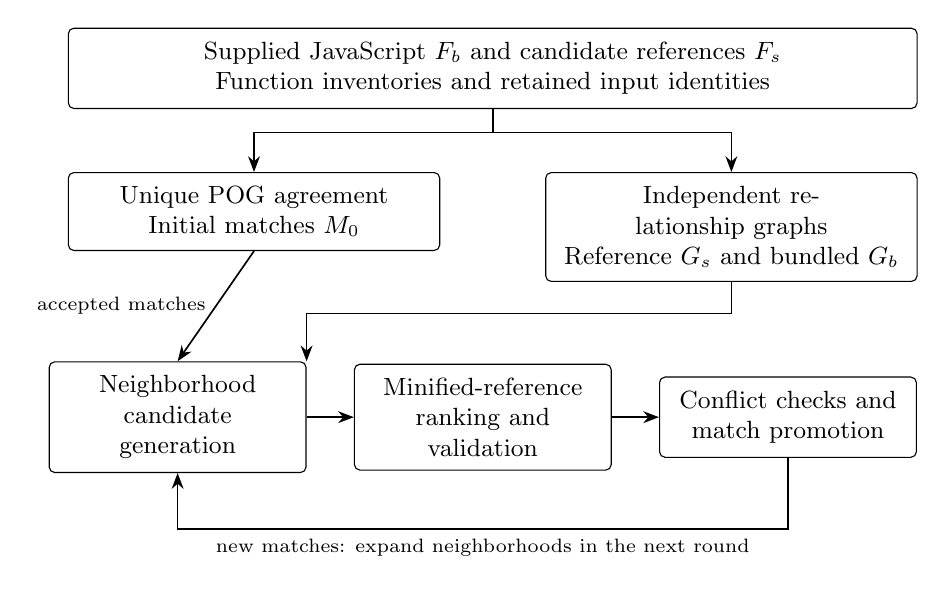
\begin{tikzpicture}[
  box/.style={draw,rounded corners=2pt,align=center,font=\small,inner sep=5pt},
  flow/.style={-{Stealth[length=2mm]},semithick}]
\node[box,text width=.86\linewidth] (input) {Supplied JavaScript $F_b$ and candidate references $F_s$\\Function inventories and retained input identities};
\node[box,text width=.36\linewidth,below=8mm of input.south,xshift=-.25\linewidth] (anchors) {Unique POG agreement\\Initial matches $M_0$};
\node[box,text width=.36\linewidth,below=8mm of input.south,xshift=.25\linewidth] (graphs) {Independent relationship graphs\\Reference $G_s$ and bundled $G_b$};
\node[box,text width=.24\linewidth,below=14mm of anchors,xshift=-.08\linewidth] (candidates) {Neighborhood\\candidate generation};
\node[box,text width=.24\linewidth,right=6mm of candidates] (rank) {Minified-reference ranking and validation};
\node[box,text width=.24\linewidth,right=6mm of rank] (promote) {Conflict checks and match promotion};
\draw[flow] (input.south) -- ++(0,-3mm) -| (anchors.north);
\draw[flow] (input.south) -- ++(0,-3mm) -| (graphs.north);
\draw[flow] (anchors.south) -- node[left,font=\scriptsize] {accepted matches} (candidates.north);
\draw[flow] (graphs.south) -- ++(0,-4mm) -| (candidates.north east);
\draw[flow] (candidates) -- (rank);
\draw[flow] (rank) -- (promote);
\draw[flow] (promote.south) -- ++(0,-9mm) -| node[pos=.25,below,font=\scriptsize] {new matches: expand neighborhoods in the next round} (candidates.south);
\end{tikzpicture}
\caption{ReCall's recovery workflow. POG anchors initialize the accepted mapping; promoted proposals supply matches for subsequent neighborhood searches.}
\label{fig:webpage-workflow}
\end{figure}

\paragraph{Running example.}
In Figure~\ref{fig:recovery-example}, assume that the omitted statements establish the POG anchor $(\texttt{a},\texttt{render})$. The short helpers do not meet the anchor size criterion. The following stages show how imports and exports expose their relationships and how the accepted pair supports candidate search for \texttt{q}.

\begin{figure}[htbp]
\centering
\begin{minipage}[t]{.47\linewidth}
\small\textbf{Reference files}
\begin{lstlisting}[basicstyle=\ttfamily\scriptsize]
// helpers.js
export function normalize(x) {
  return x.trim().toLowerCase();
}
export function emphasize(x) {
  return x.trim().toUpperCase();
}
// app.js
import {normalize, emphasize}
  from './helpers.js';
function render(row) {
  // Other anchor statements omitted.
  return row.loud
    ? emphasize(row.title)
    : normalize(row.title);
}
\end{lstlisting}
\end{minipage}\hfill
\begin{minipage}[t]{.49\linewidth}
\small\textbf{Stylized bundled code}
\begin{lstlisting}[basicstyle=\ttfamily\scriptsize]
// Bootstrap omitted; load.d
// publishes export getters.
factories[7] = (m, e, load) => {
  load.d(e, {k:()=>q, h:()=>r});
  function q(x) {
    return x.trim().toLowerCase();
  }
  function r(x) {
    return x.trim().toUpperCase();
  }
};
const n = load(7);
function a(t) {
  // Other anchor statements omitted.
  return t.loud ? n.h(t.title)
                : n.k(t.title);
}
\end{lstlisting}
\end{minipage}
\caption{Running example of recovery across an import/export boundary. The POG anchor is assumed; the example illustrates the procedure and is not experimental evidence.}
\label{fig:recovery-example}
\end{figure}

\subsection{Function inventory and POG anchors}
\label{sec:pog-anchors}
We parse each input into an abstract syntax tree (AST), enumerate function definitions, and retain their code, file locations, enclosing definitions, lexical bindings, and property operations. Anonymous and nested functions receive separate identities. Denote the reference inventory by $S$ and the bundled inventory by $B$. These inventories include functions that are ineligible for POG anchoring.

The size criterion for POG anchoring counts syntactic property-operation occurrences in a function's own body. Member reads, writes, and object-literal property initializations contribute to the count; a compound assignment or update contributes one read/write occurrence. For example, \texttt{x.value = y.value} contributes two occurrences. Repeated operations count repeatedly. Parameter defaults and nested function bodies are excluded, and unresolved computed property names use a common placeholder. This count differs from the number of distinct properties or graph nodes.

We use the DEBUN POG backend introduced in Section~\ref{sec:background-prior-work} to extract fingerprints~\cite{kim2025debun}. Nested bodies are removed or replaced by empty function expressions before extraction. An extraction failure cannot establish an anchor. A pair enters the initial mapping $M_0$ only if both functions have at least ten property-operation occurrences, their POG fingerprints agree, and the fingerprint has a unique eligible reference definition and a unique eligible bundled definition within the target matching unit. A matching unit is the target chunk for multi-chunk analysis; the single-chunk pilot has one such unit per build.

The size threshold restricts anchoring to functions with more structural evidence, while uniqueness excludes observed fingerprint collisions. Neither condition proves identity. Functions below the threshold remain in the recovery inventory and can be matched during expansion.

\subsection{Bundler-aware relationship graphs}
\label{sec:graph-construction}
ReCall constructs $G_s=(S,E_s)$ and $G_b=(B,E_b)$ independently. Their purpose is to expose candidates around accepted matches. Edges represent modeled calls, function-valued arguments and references, direct containment, and local source-order proximity. These relationships offer complementary search directions: resolved bindings connect functions across module boundaries, while containment and proximity can supply candidates where direct call resolution is unavailable. They are not assertions that every linked pair executes together.

The construction has three steps: collect available context, normalize module operations into a shared representation, and propagate function values to emit relationships. Algorithm~\ref{alg:graphs} summarizes this procedure.

\begin{algorithm}[htbp]
\caption{Constructing graphs for neighborhood search}
\label{alg:graphs}
\begin{algorithmic}[1]
\Require Reference files $F_s$, supplied bundled files $F_b$, matching inventories $S,B$
\Ensure Reference graph $G_s$ and bundled graph $G_b$
\ForAll{$x\in\{s,b\}$}
  \State $U\gets\operatorname{CollectLocalContext}(F_x)$
  \State Parse $U$ and bind identifiers to lexical declarations
  \State $\mathcal{M},K\gets\emptyset$ \Comment{module records and value constraints}
  \ForAll{units $u\in U$}
    \State Normalize aliases, constant keys, and registry addresses
    \State $\mathcal{M}\gets\mathcal{M}\cup\operatorname{RecognizeModules}(u)$
    \State Add ordinary binding, field, and return constraints to $K$
    \State Add adapter constraints for imports and exports to $K$
  \EndFor
  \State $V\gets\operatorname{SolveToFixedPoint}(K,\mathcal{M})$ within analysis limits
  \State $E\gets\operatorname{FunctionRelations}(U,V)$
  \State Add direct containment and same-parent sibling edges to $E$
  \State Project nodes and relationships to the matching inventory $S$ or $B$
  \State $G_x\gets(\operatorname{MatchingFunctionNodes}(F_x),E)$
\EndFor
\State \Return $G_s,G_b$
\end{algorithmic}
\end{algorithm}

\subsubsection{Available context and runtime scope}
\label{sec:local-context}
Context collection is independent of target selection. A supplied runtime helper can explain an export operation even if the helper itself is not a matching target. Starting from the files listed in each input manifest, the collector follows relative ESM imports and reexports, literal dynamic imports, local CommonJS requests, and statically specified module URLs only within declared local roots. It records missing files and unresolved requests. Computed chunk loading requires the relevant files to be supplied explicitly. The collector does not execute bundle code.

Module identities are scoped by environment and loader or registry. Equal numeric IDs in independent runtimes must not merge. Explicit annotations and supported worker-entry forms establish these scopes; unknown scope information remains a limitation of the input. Context code supplies constraints, while function-node emission is projected to the chosen matching inventory. This distinction lets runtime initialization/export code assist recovery without first matching its initialization functions.

\subsubsection{A shared module and function-value representation}
Building on D-Bundlr's module-analysis decomposition~\cite{xu2026dbundlr}, ReCall recognizes runtime structures, binds factory parameters to module operations, and resolves imported values. These operations produce relationships for candidate search.

For a factory with identifier $i$ in scoped registry $\rho$, the adapter creates $\mathcal{M}[\rho,i]$, containing its module object, initial exports object, and loader identity. The abstract state also contains lexical value slots, function/class tokens, allocation-site objects, and constant-key property slots. Ordinary assignments and adapter operations propagate values between these slots. Table~\ref{tab:module-operations} shows how several emitted forms feed the same representation.

\begin{table}[htbp]
\caption{Representative operations in the common module/value model.}
\label{tab:module-operations}
\centering\small
\begin{tabular}{@{}p{.29\linewidth}p{.65\linewidth}@{}}
\toprule
Operation & Modeled effect\\
\midrule
Factory registration & Allocate a module record under its scoped registry and ID; bind module/exports/loader parameter roles.\\
\addlinespace
Export assignment & Replace the modeled export value for \texttt{module.exports}, or populate a property for \texttt{exports.name}.\\
\addlinespace
Export getter & Transfer the getter's returned value to the published property.\\
\addlinespace
Constant-ID load or import & Transfer the selected module's export or namespace value to the importing binding.\\
\addlinespace
Call through a resolved value & Emit a relationship from the enclosing function to the modeled function target.\\
\bottomrule
\end{tabular}
\end{table}

In the running example, the reference import binds \texttt{normalize} to its definition. On the bundled side, \texttt{load(7)} selects the scoped module record, and the getter for \texttt{k} transfers the function token for \texttt{q} to that record's export property. Resolving \texttt{n.k(...)} consequently exposes the relationship from \texttt{a} to \texttt{q}. Module registration alone would not resolve this function-level connection.

The common solver propagates aliases, object fields, selected class members, imports, exports, and small return summaries. The summaries specialize direct parameter returns, constant member paths from parameters, and returned function/class values at individual call sites. They handle common identity and interop helpers without propagating every argument through every application function. Relationships are emitted for uniquely modeled callable values, with function-valued arguments and binding references recorded separately and opaque native alternatives retained. Flow-insensitive and accessor approximations can add neighbors. This is an incomplete candidate graph, not an exact or sound JavaScript call graph.

\subsubsection{Adapters for emitted mechanisms}
\label{sec:bundler-adapters}
Adapters normalize loading and export protocols into this shared model. They target structural roles rather than application names, library names, chunk hashes, or fixed local-variable spellings. Table~\ref{tab:bundler-mechanisms} summarizes the supported families. For scope-hoisted code, adapters use surviving lexical and ESM bindings without reconstructing erased module boundaries.

\begin{table}[htbp]
\caption{Bundler mechanisms normalized into the shared module/value model.}
\label{tab:bundler-mechanisms}
\centering\small
\begin{tabular}{@{}p{.19\linewidth}p{.34\linewidth}p{.39\linewidth}@{}}
\toprule
Family & Emitted relationship & Resolution strategy\\
\midrule
webpack/Rspack & Factory tables, scoped loaders, registered chunks & Bind module/exports/require roles; resolve constant IDs and export getters.\\
\addlinespace
esbuild/Rollup & Flattened bindings and ESM chunk imports & Follow lexical declarations and ESM namespaces; summarize retained CJS/interop helpers.\\
\addlinespace
Rolldown & ESM links, lazy CJS factories, shared runtime helpers & Allocate exports per lazy factory; interpret thunk results and getter namespaces.\\
\addlinespace
Turbopack & ID/factory registrations and context APIs & Resolve require/namespace operations and published export bindings.\\
\addlinespace
Parcel & Scope-hoisted code or loader-specific registrations & Resolve lexical links and loader-scoped factory exports; model default interop.\\
\bottomrule
\end{tabular}
\end{table}

Section~\ref{sec:bundler-selection} gives the survey-based selection rule. Appendix~\ref{sec:graph-details} preserves the individual runtime cases and bounded-worklist implementation. Those bounds control analysis cost and report incomplete analysis explicitly; they do not establish a linear-time complexity bound or complete recovery.

\subsection{Neighborhood candidate generation}
\label{sec:neighborhoods}
Accepted matches connect the two graphs for candidate search. Let $M$ map bundled functions to reference functions accepted before the current round, and let $N_s$ and $N_b$ denote undirected one-hop neighborhoods. Traversing both directions allows callers, callees, and other linked definitions to seed a search. The one-hop restriction keeps each expansion local; successive rounds can advance farther as new matches are accepted. Source-order proximity connects definitions at most two positions apart with the same immediate parent, with top-level functions grouped separately for each file.

For an unmatched bundled function $b$, let $U_M(b)$ contain reference identities already allocated in its target matching unit. In a single-chunk run, $U_M(b)=\operatorname{range}(M)$. The structural candidate pool is
\begin{equation}
\label{eq:candidate-neighborhood}
C(b)=\left(\bigcup_{b'\in N_b(b)\cap\operatorname{dom}(M)}N_s(M(b'))\right)
\setminus U_M(b).
\end{equation}
A function without a matched bundled neighbor is not examined. Otherwise, reference neighbors of the accepted counterparts supply its candidates. Taking their union avoids requiring every approximate relationship to agree, but can admit additional wrong candidates. Ranking and validation must handle that ambiguity.

For \texttt{q} in Figure~\ref{fig:recovery-example}, its accepted neighbor \texttt{a} maps to \texttt{render}. Both \texttt{normalize} and \texttt{emphasize} are neighbors of \texttt{render}, so both enter $C(\texttt{q})$ if unallocated. If either the reference import or bundled export remains unresolved, the required corresponding connection can be absent and prevent this expansion.

One-to-one allocation is scoped to the target chunk, so a reference definition may be recovered in several chunks. Within-chunk expansion restricts supporting bundled neighbors to the same chunk. The cross-chunk variant also admits statically resolved relationships to accepted functions in other supplied chunks; it does not copy matches solely because they share a reference identity. Context availability and permission to expand across chunks are separate choices.

The jQuery model pilot uses the original local graph of lexical calls, function arguments, containment, and sibling proximity. Section~\ref{sec:rq2} evaluates the extended graph separately through oracle-assisted reachability.

\subsection{Candidate ranking and validation}
\paragraph{Minified reference representations.}
ReCall minifies each reference function $s$ to obtain $m(s)$ before embedding. This representation reduces syntactic differences caused by identifier renaming and compact expressions, while retaining the original function for validation and reporting. Terser compresses the function within a temporary top-level constant; the resulting root function is extracted by its AST range and the wrapper removed. Compression uses two passes and local identifier mangling, with top-level optimization and mangling disabled. External names remain unchanged because enclosing declarations are unavailable. Isolated minification is a comparison aid, not a reconstruction of the full bundling context.

\paragraph{Bounded candidate ranking.}
We embed $m(s)$ with \texttt{qwen3-embedding:0.6b} using the semantic-comparison instruction in Appendix~\ref{sec:prompt}; bundled functions are embedded as code only. Cosine similarity orders eligible candidates in $C(b)$, with reference inventory order breaking ties. Vectors are cached by their distinct inputs. At most five candidates proceed to validation. This bounds validation work per query state, while allowing the correct identity to rank below another candidate. A correct candidate outside the shortlist cannot be recovered by that query, and similarity alone never accepts a match.

Expansion excludes reference or bundled functions longer than 18,000 JavaScript string code units before embedding; such functions may still obtain POG matches. Admitted bodies are not silently truncated. Minification failures remain explicit rather than yielding a substituted reference representation. These restrictions bound the implemented comparison procedure, not recoverability in principle.

\paragraph{Validation as a heuristic judgment.}
Here \emph{validation} means a model's assessment of a candidate pair under the adopted comparison policy. It is neither a semantic-equivalence proof nor an independent confirmation of reference identity. Each request to \texttt{qwen3.5:27b} contains the complete reference function $s$, its minified reference $m(s)$, and the bundled function $b$. Captured initializers, neighbor code, oracle names, and counterpart labels are not included. The prompt asks the model to map parameters, locals, and external variables between the bodies and compare their behavior; it permits inferred renaming of external bindings even when their declarations are absent.

The prompt illustrates compact JavaScript rewrites, including comma expressions, short-circuit and complementary conditions, operand-valued logical operators, implicit returns, and nullish coalescing. It instructs the model to reject only on clear evidence of a difference and otherwise accept, explicitly excluding corner cases and side effects. These are substantive limits of the implemented policy. Behaviorally compatible helpers can still have different reference identities, and missing binding context can make a plausible correspondence wrong. Section~\ref{sec:limitations} analyzes the observed failures.

The response must be uppercase \texttt{T} or \texttt{F}; thinking is disabled, and no variable mapping or explanation is returned. Whitespace is trimmed before strict parsing. Other outputs and API errors never count as acceptance. In the running example, the visible \texttt{toLowerCase}/\texttt{toUpperCase} difference offers evidence against pairing \texttt{q} with \texttt{emphasize}. If validation accepts \texttt{normalize}, the pair becomes a proposal, subject to the next stage's allocation checks.

\subsection{Conflict resolution and iterative expansion}
For each query, validation follows rank order and stops at the first \texttt{T}. Exhausting the selected candidates produces no proposal; invalid responses and errors allow checking the next candidate. First-positive stopping saves subsequent checks after an acceptance, but makes ranking and false acceptance consequential: lower-ranked candidates are not compared once a proposal exists. The procedure does not require a unique positive judgment across the shortlist.

\begin{algorithm}[htbp]
\caption{Iterative matching with minified references}
\label{alg:recovery}
\begin{algorithmic}[1]
\Require Reference functions $S$, bundled functions $B$, graphs $G_s,G_b$, initial anchors $M_0$
\Ensure Partial mapping $M$, one-to-one within each matching unit
\State $M\gets M_0$
\State Prepare minified references; cache embeddings as functions are queried
\Repeat
  \State $P\gets\emptyset$ \Comment{$M$ is fixed during this round}
  \ForAll{eligible unmatched $b$ with a matched neighbor}
    \State $C\gets$ eligible unused reference neighbors from Equation~\ref{eq:candidate-neighborhood}
    \If{$C\neq\emptyset$ and this candidate/neighbor state is new}
      \State $T\gets$ up to five candidates ranked by cosine similarity
      \ForAll{$s\in T$ in rank order}
        \If{$\operatorname{Validate}(s,m(s),b)=\texttt{T}$}
          \State Add $(b,s)$ to $P$
          \State \textbf{break}
        \EndIf
      \EndFor
    \EndIf
  \EndFor
  \State Remove proposals with duplicate or already used reference identities in their unit
  \State $M\gets M\cup P$
\Until{$P=\emptyset$}
\State \Return $M$
\end{algorithmic}
\end{algorithm}

The mapping $M$ stays fixed during a round. At the round's end, all proposals sharing a reference identity within a matching unit are rejected, as are proposals for an already allocated reference identity. Remaining proposals extend $M$ and supply new neighborhoods in the next round. This avoids resolving competing proposals by traversal order, but does not identify which conflicting proposal, if any, was correct.

One-to-one allocation prevents a reference definition from explaining several targets in the same chunk under the current matching policy. It is an algorithmic restriction, not a property guaranteed by JavaScript bundling. It cannot recover multiple bundled copies of one reference definition within that unit, and an incorrect allocation can exclude a later correct candidate. Accepted matches are not automatically retracted. These consequences are retained in evaluation rather than treated as evidence that the affected targets lack counterparts.

Algorithm~\ref{alg:recovery} repeats this process. A query can be reconsidered when its candidates or matched neighbors change; identical states are skipped, and complete validator requests are cached with model digests and settings. If the running example's $(\texttt{q},\texttt{normalize})$ proposal passes the conflict checks, its neighbors become usable in the following round.

Each nonterminal round adds at least one previously unmatched bundled function, so unrestricted iteration terminates on a finite inventory. A fixed point means that the procedure adds no further match under its candidate and acceptance rules, not that every target has been recovered. Configured budget stops are reported separately from convergence. The output retains accepted correspondences, their anchor or model origin, supporting matches, and reference allocations so that subsequent analysis can inspect both recovery and error propagation.


\section{Dataset Preparation}
\label{sec:datasets}
\suppressfloats[t]
This section documents the completed model fixture and graph cohorts, defines identity labels, and specifies the local verification inputs for the seven planned experiments in RQ1--RQ3. The primary recovery evaluation takes supplied JavaScript and fixed, versioned references; automatic library identification and reference retrieval are input preparation, not evaluated contributions. Source maps are withheld from model-driven recovery. The separate graph simulations use an explicitly declared oracle. The practical-use dataset for RQ4 remains to be defined.

\subsection{Completed model fixture}
\label{sec:model-fixture}
The model pilot uses a crafted task-board application and the published jQuery~4.0.0 ESM distribution. Three evaluated browser builds use esbuild~0.25.9, Rollup~4.50.0, and webpack~5.97.1 with minification enabled and tree shaking disabled. The distribution contains 558 reference definitions, and the three builds provide 1629 supported jQuery occurrences. These inputs were used during method development and are not an unseen-repository evaluation. Appendix~\ref{sec:pilot-setup} preserves build settings, model deployments, and the original experimental procedure.

\subsection{Completed graph cohorts and bundler coverage}
\label{sec:bundler-selection}
The completed oracle-assisted graph experiment extends beyond the crafted jQuery fixture. The selection is motivated by the State of JavaScript 2025 build-tool usage ranking~\cite{stateofjs2025}. We prioritize the dedicated bundler entries: webpack, esbuild, Rollup, Turbopack, Parcel, Rolldown, and Rspack (Table~\ref{tab:bundler-usage}). The survey also lists compilers, wrappers, and runtimes; we do not count them as additional dedicated bundler families. Vite's 84\% published usage motivates coverage of its backends: earlier Vite versions combine esbuild and Rollup, whereas Vite~8 adopts Rolldown~\cite{vite8}. This is a rationale for protocol coverage, not an estimate of production deployment share or a probability sample of applications.

\begin{table}[t]
\caption{Dedicated bundler entries ordered by published State of JavaScript 2025 usage ratios~\cite{stateofjs2025}. Percentages retain the survey API\textquotesingle s rounded ratios. Usage means having used a tool, not current production market share.}
\label{tab:bundler-usage}
\centering\small
\begin{tabular}{lr@{\qquad}lr}
\toprule
Bundler & Usage (\%) & Bundler & Usage (\%)\\
\midrule
\nolinkurl{webpack} & 87 & \nolinkurl{parcel} & 26\\
\nolinkurl{esbuild} & 54 & \nolinkurl{rolldown} & 10\\
\nolinkurl{rollup} & 47 & \nolinkurl{rspack} & 7\\
\nolinkurl{turbopack} & 28 &  & \\
\bottomrule
\end{tabular}
\end{table}


We retain three distinct cohorts. An earlier esbuild graph study evaluates three pinned Angular applications and 25 repository/library cases (7497 supported pairs). The current analyzer's development cohort contains eight Rspack, Rolldown, Turbopack, and Parcel applications, with 69 cases (62 having supported targets) and 161,329 supported pairs. These repositories were used while developing the adapters. The new-repository cohort freezes the analyzer before evaluation and selects five previously untested repositories: \nolinkurl{ionic-team/ionic-conference-app}, \nolinkurl{geeker-admin/Geeker-Admin}, \nolinkurl{robustmq/robustmq-copilot}, \nolinkurl{decolua/9router}, and \nolinkurl{cobiwave/simplefolio}. It covers one repository per non-webpack family, with 41 cases (40 having supported targets) and 28,780 supported pairs. The cohorts are reported separately, and the earlier esbuild implementation is not pooled with the current revision. Rollup and webpack additionally occur in the controlled jQuery builds; they are not new-repository subjects in this experiment.

We select at most ten loaded packages per application by deduplicated, source-map-embedded JavaScript-family source bytes, before inspecting recovery outcomes. The established exclusions remove the selected Angular, React, and Vue framework runtimes and build loaders. Component libraries such as Ionic and Element Plus remain in scope; this operational boundary is not a universal framework/library taxonomy. Only emitted packages count: a dependency declared but absent from bundled JavaScript does not become a test library. Simplefolio consequently contributes only vanilla-tilt. Artifacts include supplied lazy, shared, and runtime chunks within the selected browser or renderer build, rather than only the files reached by a navigation trace. Separate service-worker scripts are excluded from the new-repository browser scope.

Every subject retains a pinned commit, exact JS/map hashes, build configuration, selected packages, and input inventory. Existing corpus artifacts are reused where available. Geeker Admin is built with native Vite~8.0.16 and source maps; RobustMQ uses native Rsbuild~1.4.1 with a configuration wrapper enabling JavaScript source maps; Simplefolio uses native Parcel~2.8.2. For 9router, the pinned application script uses webpack, so we explicitly rebuild it with Next~16.3.5's Turbopack backend. Its existing build configuration emits browser maps. Google Fonts fetching failed; the successful isolated offline build uses Next's mock-response hook to substitute an empty CSS response for the Inter font URL. This omits font assets without editing application JavaScript. Failed attempts, the fixture, and the effective configuration are preserved. We therefore describe this subject as a build-adjusted Turbopack experiment, rather than an untouched default release.

These completed graph cohorts use source-map-selected references and supplied emitted artifacts. Their oracle-assisted design is specified in Section~\ref{sec:connectivity-design}. The development cohort cannot be relabeled as unseen; only the five-repository graph check freezes the analyzer before subject evaluation. None of these graph cohorts constitutes a completed model-driven recovery evaluation on unseen repositories.

\subsection{Identity labels and measurement units}
\label{sec:identity-measurements}
The following source-map policy defines assessable identities in the completed experiments and will be retained for the planned verification evaluation. In model-driven runs, the oracle labels accepted matches for scoring; it does not supply candidates or correct model decisions.

For each mapping segment, we locate the innermost bundled function containing its generated position. We retain only positions inside that function's own body, excluding the function header and the opening and closing brace positions. Expression-bodied arrows retain the full expression interval. Nested functions receive their own mapping points rather than contributing them to an enclosing function. Original positions then vote for the innermost reference function containing them.

A bundled function receives a supported reference identity when at least two retained points vote for the same reference function, its votes account for at least 80\% of all retained mapped points, and it is the unique highest-vote function. We also retain sufficiently supported application or bundler-runtime origins; predicting a library identity for one of these functions counts as wrong. A function without a supported identity or non-library origin remains unresolved. A predicted match on such a function is unassessed, rather than being silently counted as correct or wrong.

The oracle supports positional identity, not formal semantic equivalence. A different reference identity can still implement equivalent behavior. Conversely, a source-linked function can undergo a behavior-preserving specialization that changes its behavior outside the actual calling context. Our measured errors concern recovering reference identities under this oracle. Functions created by the build without a supported reference counterpart are outside the target population; their library authorship is not inferred from appearance.

Let $D$ denote supported occurrences of the selected library functions, and let $C$, $W$, and $U$ denote correct, wrong, and unassessed accepted matches. Recovery is $C/D$; assessed identity precision is $C/(C+W)$, with $U$ reported separately. Wrong library assignments to supported application or runtime functions contribute to $W$ even though those functions are outside $D$. We retain reference inventory size, parsing failures, and unsupported or ambiguous transformations so that exclusions remain visible. Distinct reference identities, bundled occurrences, library cases, repositories, and website findings have different denominators. Report per-library and per-bundler results, macro summaries, and pooled counts without treating repeated occurrences as independent trials.

\subsection{Planned verification dataset}
\label{sec:planned-verification}
The planned local dataset will cover different bundlers and target libraries/frameworks for experiments~1--5. Target packages, exact versions, framework-runtime inclusion, and supplied artifact scope will be selected before inspecting recovery outcomes. Existing exclusions in the completed graph cohorts remain unchanged and will not be treated as framework recovery results. Configuration selection for experiments~6--7 will use repository-disjoint development subjects, and the analyzer, models, prompts, and thresholds will be frozen before held-out testing. Dataset sizes, selected repositories, and preparation outcomes remain pending. Existing development subjects will retain their development status.

For each repository, we will preserve its commit, dependency lockfile, effective bundler configuration and version, browser or renderer build, and JS/map hashes. The declared local artifact set will identify entry, lazy, shared, and runtime chunks and their execution environments. All compared conditions within an experiment will use the same supplied files and local context. Locally emitted artifacts will not be described as browser-intercepted code or as complete runtime coverage. Source maps and manual review labels will be stored separately from recovery inputs.

Versioned references will be prepared from the repository's pinned dependencies and corresponding published distributions, with package variants, integrity metadata, and file hashes retained. The reference set will be fixed before recovery and shared across compared configurations. Missing or incompatible reference artifacts will be recorded as preparation exclusions, together with their affected packages; evaluation labels will not silently repair inputs. This design measures function recovery conditional on the declared references, not automatic package identification or retrieval.

For the planned boundary characterization in Section~\ref{sec:boundary-characterization}, we will retain contributor relations separately from the dominant-identity oracle above and include generated top-level regions when reviewing no-target candidates. Each source inventory will state whether it covers complete build inputs or only map-embedded source texts; unrepresented modules and unavailable source contents will limit the claimed population. No source-map absence alone will establish removal. The resulting manually validated counts will be linked to each library/build case's recovery measurements.

\subsection{Practical-use dataset: to be filled}
\label{sec:planned-websites}
The application task, dataset, and evaluation protocol for RQ4 remain to be filled. No website population, downstream comparison, or practical-use result is specified by the current roadmap.

\section{Evaluation}
\label{sec:experiment}
\label{sec:results}
The evaluation follows four research questions. RQ1 measures recovery performance across local builds from different bundlers, libraries, and frameworks, and examines the relationship between function transformations and library recovery rate. RQ2 ablates neighborhood ranking and module graph building. RQ3 studies the tradeoffs introduced by the POG feature-count threshold and validation model selection. RQ4 reserves the practical-use evaluation; its research question and experimental protocol remain to be filled.

\paragraph{Completed evidence and planned work.}
Table~\ref{tab:evidence-status} separates completed evidence from the seven planned experiments, numbered consistently with the experiment repository's roadmap. Within RQ1--RQ3, completed results precede the planned experiments. The model pilot, graph simulations, and validator comparison retain their original subjects and settings. Oracle-assisted graph reachability is reported separately from model-driven recovery. This preliminary evidence does not complete the seven planned experiments, and RQ4 has no completed practical-use result.

\begin{table}[htbp]
\caption{Evaluation status. Planned studies have no results in this draft.}
\label{tab:evidence-status}
\centering\small
\begin{tabular}{@{}p{.07\linewidth}p{.43\linewidth}p{.44\linewidth}@{}}
\toprule
RQ & Completed evidence & Planned experiment\\
\midrule
RQ1 & Known-reference jQuery model pilot with the original local graph. & (1) Different bundlers; (2) different libraries/frameworks; (3) validated function transformations and their relationship with library recovery rate.\\
\addlinespace
RQ2 & Pilot expansion and oracle-assisted graph reachability on documented repository cohorts. & (4) Neighborhood ranking versus embedding every function; (5) local versus module-aware graph building.\\
\addlinespace
RQ3 & Joint procedure/runtime comparison and controlled 27B/4B deployment comparison. & (6) POG feature-count robustness; (7) validation model correctness and cost, including end-to-end effects.\\
\addlinespace
RQ4 & None. & Practical use: to be filled.\\
\bottomrule
\end{tabular}
\end{table}

\paragraph{Shared design for planned experiments.}
Experiments~1--5 will use the local verification inputs and fixed, versioned references specified in Section~\ref{sec:planned-verification}. Complete-method runs can supply RQ1's recovery measurements and the full-method condition for both RQ2 ablations. Experiments~6--7 will use separate development subjects to select thresholds and model settings before the held-out evaluation; the selected setting's test costs can then be reused from RQ1. Comparisons will retain the same input population, identity labels, and denominator policy within each experiment. The global-embedding condition is an internal baseline for neighborhood ranking. The practical-use task, dataset, and protocol for RQ4 remain undefined.

\subsection{RQ1: Performance}
\label{sec:rq1}
\textit{How does ReCall perform across local builds from different bundlers, libraries, and frameworks, and how are function transformations related to library recovery rate?} We measure correct recovery, assessed identity precision, wrong and unassessed mappings, and computational cost using the units in Section~\ref{sec:identity-measurements}. The three planned experiments separately characterize bundler coverage, library/framework coverage, and split, combine, and remove transformations.

\subsubsection{Completed evidence: jQuery model recovery}
These completed results use the known-version jQuery fixture and original local graph (Section~\ref{sec:model-fixture}). All three builds reach a fixed point.

The reference distribution contains 558 static definitions: 85 (15.23\%) have at least ten own-body property-operation occurrences, 393 have one to nine, and 80 have none. These are implementation instances, not distinct implementation patterns. Eligibility alone does not establish a stable or unique fingerprint.

\begin{table}[htbp]
\caption{Experiment 4: correct source-identity recovery. POG counts are initial correct matches; unassessed promotions are excluded from assessed precision. The pooled row repeats source functions across builds.}
\label{tab:exp4-recovery}
\centering\small
\begin{tabular}{lrrrrrr}
\toprule
Bundler & Targets & POG & Correct & Recovery & Wrong & Unassessed\\
\midrule
esbuild & 545 & 85 & 514 & 94.31\% & 7 & 13\\
Rollup & 544 & 77 & 504 & 92.65\% & 6 & 14\\
webpack & 540 & 76 & 520 & 96.30\% & 1 & 18\\
Pooled & 1629 & 238 & 1538 & 94.41\% & 14 & 45\\
\bottomrule
\end{tabular}
\end{table}


Table~\ref{tab:exp4-recovery} separates initial POG matches from final recovery. The builds contain 568, 568, and 577 total function definitions, respectively. Of these, 545, 544, and 540 have supported jQuery identities and form the recovery denominators. Matching nevertheless retains all definitions, including application and runtime code.

Initial POG matching supplies 85, 77, and 76 correct anchors. Expansion adds 429, 427, and 444 correct matches. Final recovery ranges from 92.65\% to 96.30\%. The descriptive pooled result is 1538/1629 supported bundled-function occurrences (94.41\%), including 1300 correct matches beyond the 238 initial POG correspondences. There are 14 wrong identities and 45 unassessed promotions. Repeated occurrences across builds are correlated. Across configurations, 541 distinct reference identities are correctly recovered; this uses the 558-definition reference inventory as its denominator and must not be confused with bundled-target recovery.

\paragraph{Validation and final identity accuracy.}

\begin{table}[htbp]
\caption{Experiment 4: validation checks and assessed identity precision. Checks include repeated exact-request cache hits.}
\label{tab:exp4-validation}
\centering\small
\begin{tabular}{lrrrrr}
\toprule
Bundler & Checks & Accepted & Pair precision & Final precision & Top-5 recall\\
\midrule
esbuild & 1082 & 483 & 94.89\% & 98.66\% & 87.32\%\\
Rollup & 1125 & 515 & 92.02\% & 98.82\% & 88.81\%\\
webpack & 755 & 487 & 97.23\% & 99.81\% & 94.99\%\\
\bottomrule
\end{tabular}
\end{table}


Table~\ref{tab:exp4-validation} distinguishes precision among assessable accepted pairs from precision of final matches. The procedure performs 2962 pair checks using 2286 distinct fresh requests and 676 exact-request cache hits. All responses satisfy the T/F contract; no API error or thinking text is recorded. Among 1485 accepted checks, 1363 agree with supported reference identities, 77 disagree, and 45 are unassessed. Assessed accepted-pair precision is 1363/1440 (94.65\%), rather than 1363/1485. Repeated checks are not independent trials.

Across attempted assessable pairs, there are 1363 true positives, 68 false negatives, 77 false positives, and 1363 true negatives under the identity-label policy. These counts concern candidates actually examined, not arbitrary function pairs. Final assessed identity precision is 1538/(1538+14), or 99.10\%. Initial POG matches, repeated-query outcomes, and one-to-one filtering explain why pair and final-match denominators differ; a positive judgment alone is not the final output.

Top-five recall is conditional on attempted queries with a supported counterpart. A function may contribute several queries as its matched neighborhood changes. Of the 1300 correct model-promoted matches, 1104 were accepted at rank one, 132 at rank two, 36 at rank three, 12 at rank four, and 16 at rank five. Thus, 28 correct promotions occur at ranks four or five in their saved queries. This is an observed distribution, not an isolated estimate of the gain from increasing the validation budget.

\paragraph{Remaining failures.}

\begin{table}[htbp]
\caption{Exclusive observed outcomes for supported targets not correctly recovered. $K=3$ in experiment 3 and $K=5$ in experiment 4. Wrong promotions are already included in the totals.}
\label{tab:exp4-barriers}
\centering\small
\begin{tabular}{p{0.64\linewidth}rr}
\toprule
Observed outcome & Exp. 3 & Exp. 4\\
\midrule
Correct top-$K$ pair rejected & 274 & 21\\
Correct acceptance blocked by identity conflict & 10 & 17\\
Correct candidate outside top $K$ & 83 & 16\\
Correct pair skipped after earlier acceptance & 9 & 15\\
Wrong source promoted & 5 & 14\\
No matched neighbor & 75 & 6\\
Correct source never a candidate & 3 & 1\\
Input-size restriction & 1 & 1\\
Correct pair only invalid/error & 4 & 0\\
Total & 464 & 91\\
\bottomrule
\end{tabular}
\end{table}


Table~\ref{tab:exp4-barriers} assigns an exclusive outcome to each of the 91 supported targets not correctly recovered. Wrong promotion takes precedence; the other outcomes inspect all saved queries. The largest categories are explicit rejection of a correct top-five pair (21), an accepted correct pair blocked by a reference-identity conflict (17), a correct candidate never entering the top five (16), and early acceptance preventing validation of a correct top-five candidate (15). Six targets lack a matched neighbor. One exceeds the input limit and one never has its correct reference in a candidate pool. The 14 wrong promotions are included in the 91, not added to it.

These are observed outcomes, not additive estimates of gains from repairs. Changing a match changes later neighborhoods and reference availability. The decrease in unmatched-neighbor failures from 75 to six is consistent with greater expansion coverage, but does not isolate graph stability or the effect of an individual component.

The detailed review of all 14 wrong identities is retained in Appendix~\ref{sec:wrong-identities}.

\subsubsection{Planned experiment 1: different bundlers}
\label{sec:rq1-bundlers}
We will apply the complete method, including the extended relationship graphs, to local repository builds produced by different bundlers. The verification cohort will be held out from configuration selection, with references and input conditions fixed in advance. We will report recovery, assessed precision, wrong and unassessed mappings, runtime, and model calls per bundler, with macro summaries and pooled counts. Where the same subject can be built with multiple bundlers, we will retain paired comparisons; comparisons between different applications will be described as cohort differences rather than isolated bundler effects. Failure analysis will distinguish absent matched neighbors, missing or poorly ranked candidates, model decisions, and allocation conflicts.

\subsubsection{Planned experiment 2: different libraries and frameworks}
\label{sec:rq1-libraries}
Using local builds and exact versioned references, we will evaluate different libraries and frameworks and report the same recovery and cost measures per target package. Package selection and the inclusion of framework runtimes will be declared before observing results. The framework-runtime exclusions in the completed graph cohorts remain part of those historical cohorts; they do not constitute completed framework recovery evidence. The planned evaluation will retain reference sizes, supported target counts, parse failures, and unresolved cases, and distinguish previously used subjects from held-out subjects. We will report POG size eligibility and admitted anchors separately; the planned eligibility measurement in Background remains unfilled.

\rqoverview{Local builds across\\bundlers and packages}{Run fixed method;\\validate transformations}{Recovery, precision,\\cost, and associations}{Planned RQ1 experiments 1--3: evaluate bundler and library/framework performance and relate validated transformations to recovery.}{fig:rq1-goal}

\subsubsection{Planned experiment 3: function transformations and recovery rate}
\label{sec:boundary-characterization}
We will count split, combine, and remove candidates using source-map relations, then manually validate every flagged candidate before drawing conclusions about transformation frequency. For each selected library and build, we will relate source definitions to the bundled functions receiving their mapping points. Nested bodies will be attributed to their innermost functions. We will retain all contributor votes rather than only the dominant identity used by the recovery oracle. The initial screen will require at least two mapping points per relation and report sensitivity to this threshold. Relations will be aggregated across the supplied chunks of one build; independent builds will remain separate.

\begin{table}[htbp]
\caption{Planned source-map screening for function-boundary transformations. Each relation identifies a candidate requiring manual validation.}
\label{tab:boundary-candidates}
\centering\small
\begin{tabular}{@{}p{.43\linewidth}p{.52\linewidth}@{}}
\toprule
Observed relation & Candidate interpretation\\
\midrule
One source function $\rightarrow$ multiple bundled functions & Split candidate; duplication or mapping artifacts are alternatives.\\
\addlinespace
Multiple source functions $\rightarrow$ one bundled function & Combine candidate, including inlining.\\
\addlinespace
Source function $\rightarrow$ no mapped target & Possible removal; missing mappings or surviving top-level code are alternatives.\\
\bottomrule
\end{tabular}
\end{table}

\paragraph{Manual validation.}
Review will inspect the exact source and generated code, mapping locations, and enclosing contexts. Multi-target cases will be checked for genuine partitioning versus duplicated copies or nesting artifacts; multi-source cases will be checked for combined contributions, including inlining. For no-target cases, reviewers will also inspect generated top-level regions and all supplied chunks, using build-input inventories and compiler evidence where available. A missing function definition after inlining will count as combination when its computation survives, rather than as removal. Removal requires evidence that the function's computation was eliminated. Cases without sufficient evidence will remain unresolved. Each decision will retain source/generated locations, supporting evidence, and review notes, with disagreements adjudicated explicitly. These labels will be independent of ReCall's predictions.

\paragraph{Counts and recovery consequences.}
We will report screened candidates, confirmed transformations, alternative explanations, and unresolved cases per library and bundler. Counts will identify affected source definitions per build, with bundled-function and transformation-group counts reported separately. Overlapping transformations will be marked explicitly rather than summed into an exclusive partition. The source-inventory scope, parsing failures, missing artifacts, and map coverage will accompany each denominator. Final conclusions will distinguish observed frequency from unresolved coverage and relate validated cases to ReCall's outcomes: recovery and assessed precision for surviving supported counterparts, and coverage limits where no standalone counterpart remains. Confirmed removals will be reported as build elimination rather than matcher failures. The existing supported-target recovery denominator will remain explicit; the characterization will not silently convert unsupported transformations into assessed matches or exclude them from the scope discussion.

For each library/build case, we will relate its confirmed split, combine, and remove frequencies to its library recovery rate, retaining unresolved transformation cases separately. We will compare cases within bundler and library groups where the data permit and report target counts, source-inventory coverage, and anchor coverage alongside the association. This analysis will describe relationships rather than establish that transformations alone cause differences in recovery. Rates over surviving supported targets and coverage relative to the source inventory will remain separate, since removal or loss of a standalone boundary can change the available target population.

\paragraph{Status.}
\textit{Pending: experiments 1--3 across bundlers and libraries/frameworks, validated transformation counts, and their relationship with library recovery rate. The completed jQuery pilot does not establish these broader outcomes.}

\subsection{RQ2: Ablation}
\label{sec:rq2}
\textit{How do neighborhood ranking and module graph building affect recovery quality and computational cost?} Planned experiment~4 compares neighborhood ranking with directly embedding every function and searching the full reference pool. Planned experiment~5 isolates module-aware graph building relative to local function relationships. The completed expansion and connectivity studies below provide preliminary evidence; graph reachability alone does not measure ranking, validation, or final model recovery.

\paragraph{Completed expansion evidence.}
In the jQuery pilot, final recovery includes 1300 correct matches beyond 238 correct initial POG correspondences (Table~\ref{tab:exp4-recovery}). This comparison measures expansion under the pilot's local graph. The graph simulations below separately measure the extended resolver under ideal candidate selection; their rates must not be pooled with model recovery.

\subsubsection{Completed graph experiment: protocol}
\label{sec:connectivity-design}
This experiment isolates whether the graph can expose the correct candidate. We keep the original fingerprint proposal rule, record every proposal, and admit only oracle-confirmed, unambiguous initial pairs as seeds. Incorrect and unassessed proposals are recorded and withheld. The same seeds are used for every graph variant. This sanitization is specific to simulation; it is not an extra oracle available to model-driven recovery.

Let $T$ be the fixed set of source-map-supported target pairs, $A_0\subseteq T$ the confirmed seeds, and $A_r$ the accepted pairs after round $r$. We replace both embedding ranking and model validation with an oracle selection rule:
\begin{equation}
\label{eq:oracle-connectivity}
A_{r+1}=A_r\cup\{(b,s)\in T\mid s\in C_r(b),\ b,s\text{ are eligible}\}.
\end{equation}
Here $C_r$ is Equation~\ref{eq:candidate-neighborhood} evaluated using $A_r$. The oracle selects the correct reference anywhere in the neighborhood, without a top-$k$ restriction. Eligibility retains the 18,000-code-unit promotion limit. Supported pairs with repeated reference identities within the same target chunk stay in the denominator but cannot promote or bridge. Source definitions may recur across distinct chunks. No model, embedding service, or cached model judgment is invoked.

The baseline uses the original local calls, function arguments, containment, and sibling window of two. The source-only comparison augments the reference graph while retaining the original bundled graph. The within-chunk comparison augments both graphs but permits each promotion only through a bundled neighbor in the same target chunk. The separate cross-chunk comparison additionally permits statically resolved inter-chunk relationships. Both can analyze runtime-only dependency code: context availability and permission to promote across chunks are different factors. Neither variant adds target pairs or initial anchors through those helper files, matches initialization functions as a prerequisite, or copies an anchor by reference identity alone.

The simulation iterates to a fixed point and reports $R/D$, where $R$ counts reached supported pairs and $D=|T|$. A reference function duplicated across chunks can contribute several pairs, so this is not unique-source-function recall. We retain zero-supported library cases as N/A, reference parse failures, and ambiguous transformations. Each promotion has a checked reference-side and bundled-side parent witness; independent queue and layered traversals agree on the fixed point. Exact target/seed hashes are unchanged across variants, and the new-repository run also verifies the frozen analyzer hashes. The resulting rate measures reachable correct candidates under ideal ranking and validation. It does not measure final model accuracy or prove that every graph edge is a real call.

\subsubsection{Completed graph experiment: results}
We report each cohort separately to preserve its development or test role.
\label{sec:connectivity-results}
\paragraph{Development subjects.}
Table~\ref{tab:simulation-development} reports the current graph extension on the eight development repositories. With the same targets and seeds, within-chunk reachability rises from 104,594/161,329 (64.83\%) to 157,282/161,329 (97.49\%). Cross-chunk promotion adds 550 pairs, reaching 157,832/161,329 (97.83\%). Table~\ref{tab:simulation-stages} separates source-only augmentation from augmentation on both sides. The source-only stage reaches 110,561 pairs; adding the bundled relationships reaches another 46,721. These increments are staged effects, rather than independent causal effects of individual adapter rules.

\begin{table}[t]
\caption{Development subjects: supported-pair connectivity (\%). Base uses the original local graph; Within uses the current graph with per-chunk promotion; Cross additionally permits cross-chunk promotion. All variants retain the same $D$ targets and seeds.}
\label{tab:simulation-development}
\centering\small
\setlength{\tabcolsep}{4pt}
\begin{tabular}{@{}p{.34\linewidth}lrrrr@{}}
\toprule
Subject & Family & $D$ & Base & Within & Cross\\
\midrule
\nolinkurl{vue-admin-better} & Rspack & 13,160 & 82.52 & 95.05 & 97.70\\
\nolinkurl{Motrix} & Rolldown & 16,221 & 88.54 & 97.60 & 98.38\\
\nolinkurl{cypress-realworld-app} & Rolldown & 5,548 & 73.00 & 82.93 & 82.93\\
\nolinkurl{ZyPlayer} & Rolldown & 114,389 & 57.24 & 98.83 & 98.89\\
\nolinkurl{wechat-miniapp-radar} & Turbo & 12 & 25.00 & 25.00 & 25.00\\
\nolinkurl{next-ai-draw-io} & Turbo & 8,126 & 93.61 & 96.49 & 96.49\\
\nolinkurl{github-profile-readme-generator} & Turbo & 3,835 & 57.26 & 88.92 & 88.92\\
\nolinkurl{focalboard} & Parcel & 38 & 94.74 & 97.37 & 97.37\\
\midrule
Total & & 161,329 & 64.83 & 97.49 & 97.83\\
\bottomrule
\end{tabular}
\end{table}




\begin{table}[t]
\caption{Staged graph comparisons. Values are recovered supported pairs; source-only changes the source graph while retaining the local bundled graph.}
\label{tab:simulation-stages}
\centering\small
\begin{tabular}{lrr}
\toprule
Stage & Development ($D=161{,}329$) & Holdout ($D=28{,}780$)\\
\midrule
Local graphs & 104,594 & 22,494\\
Source graph only & 110,561 & 25,637\\
Both graphs, within chunk & 157,282 & 26,402\\
Both graphs, cross chunk & 157,832 & 26,540\\
\bottomrule
\end{tabular}
\end{table}


The largest gain comes from ZyPlayer's \nolinkurl{tdesign-icons-vue-next}. Its baseline reaches 8/41,489 pairs, an intermediate graph revision reaches 1530, and the current graph reaches all 41,489 using the same four icon seeds. The intermediate input omitted an imported Rolldown runtime helper, leaving 39,959 targets inside 2352 lazy-factory groups without accepted bundled neighbors. A controlled diagnostic adds that helper as context with no matchable helper functions and recovers the 39,959 pairs while retaining the reference graph, target set, seeds, and within-chunk protocol. Automatic dependency collection supplies the same context in the current run. Resolving initialization/export behavior thus exposes relationships without first matching initialization functions.

This one library contributes 41,481 of the 52,688 additional pairs (78.7\%). Excluding it, development-cohort reachability still rises from 104,586/119,840 (87.27\%) to 115,793/119,840 (96.62\%). We therefore report the complete per-library results rather than interpreting the 97.49\% aggregate as a typical application rate (Appendix~\ref{sec:simulation-library-results}).

\paragraph{Previously untested repositories.}
The analyzer is unchanged for the five new repositories in Table~\ref{tab:simulation-holdout}. Within-chunk reachability increases from 22,494/28,780 (78.16\%) to 26,402/28,780 (91.74\%); allowing cross-chunk promotion reaches 26,540/28,780 (92.22\%). Four repositories improve, and 26 of the 40 evaluable library cases improve. The source-only stage adds 3143 pairs; bundled relationships add another 765; cross-chunk promotion adds 138. Thus, both graph sides contribute, and the gain is not confined to the missing-helper case observed during development.

\begin{table}[t]
\caption{Previously untested repositories with the analyzer unchanged: supported-pair connectivity (\%). Turbo denotes Turbopack. The Parcel subject has only 14 supported pairs.}
\label{tab:simulation-holdout}
\centering\small
\setlength{\tabcolsep}{4pt}
\begin{tabular}{@{}p{.34\linewidth}lrrrr@{}}
\toprule
Subject & Family & $D$ & Base & Within & Cross\\
\midrule
\nolinkurl{ionic-conference-app} & esbuild & 5,355 & 69.90 & 83.40 & 85.68\\
\nolinkurl{Geeker-Admin} & Rolldown & 17,675 & 85.02 & 96.10 & 96.10\\
\nolinkurl{9router} & Turbo & 2,281 & 62.91 & 80.93 & 80.93\\
\nolinkurl{robustmq-copilot} & Rspack & 3,455 & 66.14 & 89.73 & 90.19\\
\nolinkurl{simplefolio} & Parcel & 14 & 28.57 & 28.57 & 28.57\\
\midrule
Total & & 28,780 & 78.16 & 91.74 & 92.22\\
\bottomrule
\end{tabular}
\end{table}


The per-library changes include Ionic's RxJS (47/287 to 270/287), Geeker Admin's ECharts (3135/3681 to 3660/3681) and axios (222/308 to 284/308), RobustMQ's lodash (7/196 to 163/196), and 9router's Recharts (648/1267 to 1009/1267). RobustMQ's date-fns reaches 74/107 within chunks and 90/107 with cross-chunk promotion, compared with 6/107 at baseline. These examples involve lexical imports, wrapped module exports, and namespace relationships across different applications.

Some packages remain disconnected. Geeker's \nolinkurl{@element-plus/icons-vue} stays at 1/293, with 292 targets lacking an accepted bundled neighbor. RobustMQ's \nolinkurl{@radix-ui/react-icons} stays at 0/12 without initial seeds. In 9router, \nolinkurl{@reduxjs/toolkit} remains 0/114 without seeds. Simplefolio stays at 4/14: five cases are excluded from promotion by same-chunk identity ambiguity and five lack an accepted bundled neighbor. Its small emitted library population provides limited evidence about Parcel. Moreover, 85 selected reference files in 9router's \nolinkurl{@dnd-kit/core} fail parsing and yield no supported targets for that package; its N/A entry must not be interpreted as successful recovery.

\paragraph{Earlier esbuild evidence.}
The preceding esbuild graph revision improves three applications from 5763/7497 (76.87\%) to 6832/7497 (91.13\%) within chunks and 6853/7497 (91.41\%) across chunks (Table~\ref{tab:simulation-esbuild}). It supplies additional evidence for lexical/import resolution, but its different implementation revision is retained separately. The unchanged-analyzer Ionic result above provides the new-repository esbuild check for the current implementation.

\begin{table}[t]
\caption{Earlier esbuild graph experiment, retained as a separate implementation revision: supported-pair connectivity (\%). It is not pooled with the current-analyzer cohorts.}
\label{tab:simulation-esbuild}
\centering\small
\setlength{\tabcolsep}{4pt}
\begin{tabular}{@{}p{.34\linewidth}lrrrr@{}}
\toprule
Subject & Family & $D$ & Base & Within & Cross\\
\midrule
\nolinkurl{angular-realworld-example-app} & esbuild & 711 & 30.38 & 73.14 & 73.14\\
\nolinkurl{angular-example-app} & esbuild & 1,185 & 63.04 & 88.95 & 90.72\\
\nolinkurl{ngx-charts} & esbuild & 5,601 & 85.70 & 93.88 & 93.88\\
\midrule
Total & & 7,497 & 76.87 & 91.13 & 91.41\\
\bottomrule
\end{tabular}
\end{table}


\paragraph{Candidate-edge audit and interpretation.}
We inspect 55 deterministic, edge-kind-stratified added relationships and selected new-promotion witnesses from the new repositories. Fifty have supporting code/binding evidence; four getter reads are mislabeled as function arguments but retain a genuine caller/accessor dependency; one write-only assignment produces a spurious function-value reference. All edges remain in the reported experiment. This graph deliberately supplies candidates rather than certifying calls, and these observations do not trigger a precision-oriented repair in this evaluation. A separate diagnostic suppressing the syntax-screened getter-value and write-only patterns changes reachability by only one Ionic pair; that statement itself reads a getter, so the loss does not establish a false source correspondence. The small stratified audit is not an unbiased edge-precision estimate.

The results show that mechanism-based graph construction transfers to several previously untested repositories and exposes additional correct candidates. They do not establish a universal bundler recognizer or final model recovery on these expanded graphs. Broad candidate edges can increase ranking work or compete for the validation budget; actual ranking and validation remain necessary to decide identities. The earlier 94.41\% jQuery result and these oracle connectivity rates measure different stages and populations and must not be combined.

\subsubsection{Planned experiment 4: neighborhood ranking}
\label{sec:rq2-ranking}
On the same local verification subjects and fixed references as RQ1, we will compare ReCall's neighborhood ranking with a baseline that directly embeds every eligible source and bundled function. The baseline will consider every eligible unmatched bundled function and rank candidates across the full available reference-function pool, without requiring a matched graph neighbor. Both conditions will use identical initial POG anchors, embedding and validation models, prompts, top-$k$, size limits, acceptance/conflict rules, and declared resource budgets. Anchors will be admitted by ReCall's rule without oracle filtering. Thus the comparison measures the neighborhood search strategy, including which targets it reaches, rather than changing the validator.

We will compare recovery, assessed precision, wrong and unassessed mappings, embedding work, candidate comparisons, validation calls, runtime, and memory. Cost accounting will include the baseline's complete embedding preparation and identify cache reuse explicitly. Budget-limited runs will retain their stopping status and recovered counts. The full-method condition can reuse the RQ1 runs. The completed graph simulations do not provide results for this global-embedding baseline.

\subsubsection{Planned experiment 5: module graph building}
\label{sec:rq2-modules}
We will compare model-driven recovery using local function relationships with recovery using the module-aware graph. Both conditions will retain the same input files, source references, initial anchors, neighborhood ranking, validator, thresholds, and other settings. We will measure final recovery and assessed precision together with wrong and unassessed mappings, graph-construction cost, candidate breadth, model calls, and total runtime. The module-aware condition can reuse the full-method RQ1 runs. Oracle-assisted reachability will remain a separate diagnostic; the completed simulations above do not fill this model-driven ablation.

\rqoverview{Same inputs, references,\\anchors, and models}{Neighborhood vs. global;\\local vs. module graph}{Compare recovery\\quality and cost}{Planned RQ2 experiments 4--5: independently compare neighborhood ranking and module graph building.}{fig:rq2-goal}

\paragraph{Status.}
\textit{Pending: experiment 4's neighborhood-versus-global comparison and experiment 5's model-driven graph ablation. Completed pilot expansion and oracle-assisted graph reachability remain preliminary evidence for different comparisons.}

\subsection{RQ3: Tradeoff}
\label{sec:rq3}
\textit{How do the POG feature-count threshold and validation model selection trade recovery and validation quality against computational cost?} Planned experiment~6 varies anchor eligibility to assess POG robustness, anchor coverage and precision, and downstream recovery. Planned experiment~7 compares validation correctness and cost across model deployments and measures their end-to-end effects. The completed procedure and model comparisons below retain their original settings and do not complete these planned studies.

\subsubsection{Completed pilot: procedure and runtime comparison}

\begin{table}[htbp]
\caption{Experiment 4 per-build execution. Rounds include the final round without additions. Time includes bundle embedding, validation and checkpoint overhead, but excludes the shared source embedding stage.}
\label{tab:exp4-runtime}
\centering\small
\begin{tabular}{lrrrr}
\toprule
Bundler & Rounds & Fresh calls & Cache hits & Minutes\\
\midrule
esbuild & 5 & 891 & 191 & 28.83\\
Rollup & 5 & 839 & 286 & 31.44\\
webpack & 8 & 556 & 199 & 21.24\\
\bottomrule
\end{tabular}
\end{table}




\begin{table}[htbp]
\caption{Completed overall experiments on identical bundle and oracle inputs. Several method changes are combined; this is not a component ablation. Both runs start with fresh experiment caches.}
\label{tab:exp4-comparison}
\centering\small
\begin{tabular}{p{0.52\linewidth}rr}
\toprule
Measurement & Experiment 3 & Experiment 4\\
\midrule
Correct identities / supported targets & 1165/1629 & 1538/1629\\
Correct recovery & 71.52\% & 94.41\%\\
Wrong identities & 5 & 14\\
Unassessed promotions & 36 & 45\\
Assessed identity precision & 99.57\% & 99.10\%\\
Overall run time (minutes) & 179.14 & 81.84\\
Distinct validation requests & 2837 & 2286\\
Validation request time (seconds) & 7051.33 & 4731.87\\
Invalid responses / API errors & 0/5 & 0/0\\
\bottomrule
\end{tabular}
\end{table}


Experiment~4 completes matching and its scheduled evaluation in 4910.19 seconds (81.84 minutes), compared with 10748.47 seconds (179.14 minutes) for experiment~3: an observed reduction of 54.32\%. Summed validator request time is 4731.87 seconds; reference embedding takes 15.28 seconds, bundle embeddings 35.95 seconds, and reference preprocessing (including minification and input construction) 0.389 seconds. Ranking takes 0.585 seconds. API subtotals exclude other control and checkpoint overhead and do not sum to overall elapsed time. Per-build times exclude shared reference preparation. Request latency has a median of 1.419 seconds and a 95th percentile of 5.030 seconds.

Correct recovery increases by 373 occurrences and 22.90 percentage points, while distinct validation requests decrease from 2837 to 2286 (Table~\ref{tab:exp4-comparison}). Correct-pair rejection outcomes decrease from 274 to 21, and ranking misses from 83 to 16, with different top-$K$ budgets. Wrong identities increase from five to 14, and assessed precision decreases from 99.57\% to 99.10\%. The revised procedure improves observed coverage and runtime while retaining a precision cost. Several changes are combined and each timing is a single run; these results do not identify the contribution of minification, the prompt, or the larger validation budget individually.

\subsubsection{Completed pilot: changing the validator deployment}
\label{sec:4b-results}

\begin{table}[htbp]
\caption{Controlled validator comparison. Experiment 5 replaces only the 27B validator with the 4B deployment; both use the same prompt and matching rules.}
\label{tab:exp5-model-comparison}
\centering\small
\begin{tabular}{p{0.53\linewidth}rr}
\toprule
Measurement & 27B (Exp. 4) & 4B (Exp. 5)\\
\midrule
Correct identities / supported targets & 1538/1629 & 1300/1629\\
Recovery & 94.41\% & 79.80\%\\
Wrong identities & 14 & 62\\
Unassessed promotions & 45 & 38\\
Final assessed precision & 99.10\% & 95.45\%\\
Accepted-pair assessed precision & 94.65\% & 61.03\%\\
Overall time (minutes) & 81.84 & 13.00\\
Fresh validator requests & 2286 & 1517\\
Pair checks, including cache hits & 2962 & 3143\\
Invalid responses / API errors & 0/0 & 0/0\\
\bottomrule
\end{tabular}
\end{table}




\begin{table}[htbp]
\caption{Recovery by bundler with unchanged inputs. Wrong counts include known non-library functions incorrectly identified as jQuery.}
\label{tab:exp5-build-comparison}
\centering\small
\begin{tabular}{lrrrr}
\toprule
Bundler & Targets & 27B correct & 4B correct & Wrong 27B / 4B\\
\midrule
esbuild & 545 & 514 (94.31\%) & 404 (74.13\%) & 7 / 23\\
Rollup & 544 & 504 (92.65\%) & 423 (77.76\%) & 6 / 14\\
webpack & 540 & 520 (96.30\%) & 473 (87.59\%) & 1 / 25\\
\bottomrule
\end{tabular}
\end{table}


Experiment~5 correctly recovers 1300/1629 supported targets (79.80\%), including 1062 matches beyond the same 238 correct initial POG matches. Recovery decreases by 238 occurrences, or 14.61 percentage points, relative to experiment~4. There are 62 wrong identities and 38 unassessed promotions; final assessed precision decreases from 99.10\% to 95.45\% (Table~\ref{tab:exp5-model-comparison}). Recovery decreases for every bundler (Table~\ref{tab:exp5-build-comparison}). Of the 62 errors, 58 assign a wrong reference to a supported jQuery target, while four identify application functions as library functions. All 62 count against precision, but only the 58 belong to the recovery denominator.

Observed overall time decreases from 4910.19 to 780.22 seconds (81.84 to 13.00 minutes), a 6.29-fold speedup. The 4B run makes 1517 fresh validation requests and reuses 1626 exact requests, producing 3143 pair checks. Summed fresh-validator request time is 562.78 seconds. Reference and bundle embedding take 14.87 and 34.82 seconds, respectively. All responses satisfy the T/F contract; no API error or thinking text is recorded. On 1428 shared exact user requests, median request wall time is 1.542 seconds for 27B and 0.258 seconds for 4B. These timings describe the installed deployments and observed runs, not a hardware-independent effect of model size.

\paragraph{More acceptances do not imply greater recovery.}
The 4B validator accepts all 1660 evaluated correct-pair checks, but also accepts 1060 incorrect-pair checks. It rejects 333 incorrect checks; 90 checks are unassessed. Accepted-pair assessed precision is therefore 1660/(1660+1060), or 61.03\%, compared with 94.65\% for 27B. These counts include repeated, adaptively selected checks; accepting every examined correct pair does not establish recall on all possible pairs.

The models examine 1569 common bundled/reference identity pairs. For 208 incorrect pairs, 27B rejects while 4B accepts; for 21 correct pairs, 27B rejects while 4B accepts. Another 11 unassessed pairs change from rejection to acceptance. No shared pair changes from acceptance to rejection. The result supports increased permissiveness as the observed decision difference, without revealing the model's internal reason for any judgment.

\begin{table}[htbp]
\caption{Exclusive outcomes for supported targets not correctly recovered. Four additional 4B errors concern application functions and are outside this denominator.}
\label{tab:exp5-barriers}
\centering\small
\begin{tabular}{p{0.63\linewidth}rr}
\toprule
Observed outcome & 27B & 4B\\
\midrule
Correct pair skipped after earlier acceptance & 15 & 113\\
Correct acceptance blocked by identity conflict & 17 & 92\\
Wrong source promoted & 14 & 58\\
Correct candidate outside top five & 16 & 37\\
No matched neighbor & 6 & 25\\
Correct source never a candidate & 1 & 2\\
No available source candidate & 0 & 1\\
Input-size restriction & 1 & 1\\
Correct top-five pair rejected & 21 & 0\\
Total & 91 & 329\\
\bottomrule
\end{tabular}
\end{table}


Table~\ref{tab:exp5-barriers} explains the resulting loss of coverage. Early acceptance prevents checking a correct top-five candidate for 113 targets, and identity conflicts block an accepted correct candidate for 92. A further 58 targets receive a wrong reference. Because the procedure stops at the first positive and excludes allocated references from later candidate pools, an incorrect positive can obstruct a correct match even when the validator would accept that correct pair. No target is classified as a correct top-five pair explicitly rejected in this 4B run. The nine exclusive outcomes sum to 329 unrecovered or wrongly recovered supported targets. Thirteen wrong predictions also have an earlier wrong owner that has already consumed the correct reference identity; this is allocation evidence, not a measured gain from rollback.

\paragraph{Concrete wrong acceptances and review scope.}
Experiment~5 case W01 assigns a callback-producing factory to a string-replacement function. The selected reference is \texttt{createInputPseudo}; the bundled counterpart is \texttt{unescapeSelector}. W12 selects \texttt{Identity}, which returns its argument, for a callback that writes an object flag and returns implicitly. W16 and W17 identify application DOM-building and event callbacks as library selector predicates; W31 and W32 repeat these errors in Rollup. W21 confuses the enclosing \texttt{then} method with its nested \texttt{mightThrow} function. These errors include visible root behavior differences, beyond uncertainty about external variable declarations. Case IDs are local to each experiment.

Independent own-body mapping witnesses agree with all 62 stored wrong-identity labels. Requests, outputs, and code pairs are retained for every case. The preliminary structural grouping leaves 52 cases for individual review and one same-structure binding case unresolved; we do not claim complete semantic adjudication of all 62 errors. Under the fixed prompt and allocation rules, the 4B deployment provides lower latency but substantially lower recovery and identity precision. We retain 27B as the main configuration; a revised 4B prompt would require a separate evaluation.

\subsubsection{Planned experiment 6: POG feature-count robustness}
\label{sec:rq3-pog}
On repository-disjoint development subjects, we will vary the minimum number of own-body property-operation occurrences required for POG anchoring, initially comparing thresholds 5, 10, and 20 with the 27B validator fixed. References, graph construction, the 0.6B embedding model, prompts, and other settings will remain fixed. We will report eligible function counts, anchor coverage, anchor precision, fingerprint ambiguity, final recovery and assessed precision, wrong and unassessed mappings, and computational cost. This experiment changes anchor eligibility rather than the POG hashing algorithm; threshold eligibility, retained fingerprint evidence, and accepted anchors will be reported separately. The selected threshold will be frozen before the held-out RQ1 evaluation.

\subsubsection{Planned experiment 7: validation model selection}
\label{sec:rq3-validator}
We will compare validation model deployments, initially the 27B and 4B configurations, with the POG threshold held at 10 and the references, graph, ranker, prompt, and acceptance rules fixed. A shared labeled function-pair set from development subjects will measure correct acceptances, false acceptances, false rejections, invalid/error responses, and latency and resource cost. Pair selection and labels will be frozen before comparing models, with correct pairs and hard negative identities represented explicitly. These judgments measure source-identity agreement rather than formal semantic-equivalence proofs.

Separate end-to-end runs on the same development builds will measure recovery, assessed precision, wrong and unassessed mappings, allocation conflicts, model calls, and total cost under each validator. This separates comparison on identical pairs from consequences of the different search trajectories. Model digests and serving settings will be recorded, and the selected configuration will be frozen before the held-out evaluation. The chosen setting's test costs can be reused from RQ1. Recovery time will be separated from input preparation and oracle scoring; historical pilot totals retain their recorded timing boundaries.

\rqoverview{Fixed development set\\and reference inputs}{Vary POG threshold;\\compare validators}{Anchor / pair quality,\\recovery, and cost}{Planned RQ3 experiments 6--7: vary anchor eligibility and validation models separately before selecting the test configuration.}{fig:rq3-goal}

\begin{samepage}
\paragraph{Status.}
\textit{Pending: experiments 6--7 on the development dataset, including the POG threshold sweep and shared-pair validation-model comparison. The current threshold of 10 is not claimed to be optimal. The completed pilot compares only the installed validator deployments at threshold 10 on its original subject.}
\par
\end{samepage}

\subsection{RQ4: Practical Use}
\label{sec:rq4}
\textit{Practical-use research question: to be filled.} The application task, dataset, comparison conditions, and evaluation measures remain to be specified.

\paragraph{Completed evidence.}
There is no completed practical-use evaluation in this draft. The recovery and graph results in RQ1--RQ3 do not establish downstream improvement.

\paragraph{Planned experiment.}
\textit{To be filled.}

\paragraph{Status.}
\textit{Pending: definition of the practical-use research question and experimental protocol. No practical-use result is claimed.}


\section{Threats to Validity and Limitations}
\label{sec:limitations}
\paragraph{Input and reference availability.}
Recovery is conditional on supplied code and candidate references. The completed experiments and planned primary evaluation use fixed reference inputs; they do not establish the accuracy or cost of automatic package identification and retrieval. Missing dependencies, unavailable package variants, patched library copies, and uncaptured chunks can limit the available correspondences. The planned verification dataset records missing or incompatible references as preparation exclusions rather than silently repairing inputs or attributing these failures to the matcher. The RQ4 practical-use protocol remains undefined, and no downstream improvement is established in this draft.

\paragraph{Deliberate obfuscation.}
Our evaluation targets bundling and minification and does not establish robustness to deliberate JavaScript obfuscation. Prior web measurements found explicit obfuscation substantially less prevalent than minification~\cite{skolka2019anything}; these historical findings do not establish its current prevalence. Property-name concealment or renaming can invalidate POG anchors, while control-flow flattening and inserted dispatchers or wrappers can disrupt relationship graphs and candidate comparison. Packing, runtime-generated code, and virtualization may hide or replace the original function bodies, limiting the available static correspondences. We leave systematic evaluation under these transformations and extensions for recovering obfuscated functions to future work; the reported recovery and reachability results should not be generalized to such inputs.

\paragraph{Source identity versus semantic equivalence.}
Our objective is correspondence to a particular source definition. Different definitions can implement the same behavior, so a valid semantic acceptance can still disagree with this identity oracle. Conversely, a source-linked bundled function may be specialized to its actual callers and differ on unreachable inputs. We therefore describe precision as source-identity agreement, not as the probability that a semantic-equivalence proof is correct. We do not treat every identity error as an independently established semantic false positive.

\paragraph{External bindings and missing program context.}
Function bodies alone may not identify decisive enclosing bindings. Eight of the 14 wrong identities in the 27B run involve different regex/replacement helpers or public/private data stores behind nearly identical wrapper bodies. Minifying the source improves syntactic comparability but does not recover the bundled binding's origin. The permissive prompt allows inferred correspondences and accepts without a demonstrated difference. This policy can accept a plausible but wrong binding mapping. The limitation is not the mere presence of an external variable: sufficient local differences can still justify rejection. Additional binding evidence or relevant helper definitions would be needed to resolve ambiguous cases reliably.

\paragraph{Permissive validation and function boundaries.}
The adopted prompt explicitly excludes corner cases and side effects, weakening the comparison relative to full JavaScript semantics. This restriction can hide differences in data writes or helper calls, although T/F outputs do not reveal whether it caused any particular acceptance. Two wrong setter matches have different arguments and enclosing roles; another confuses a layout-test result with the jQuery object. Three more confuse enclosing functions with nested functions. Shared nested code must not establish equivalence of the root functions. Neither a larger model nor a minified reference guarantees correct boundary or behavior analysis.

\paragraph{Validator-dependent acceptance policy.}
The same permissive prompt yields accepted-pair assessed precision of 94.65\% with 27B and 61.03\% with 4B. The absence of observed correct-pair rejections in the 4B run does not make it a reliable validator: false acceptances can terminate a search early or block other proposals. First-positive stopping and one-to-one allocation can amplify this difference. We observe the decisions and their pipeline consequences, but T/F-only outputs do not establish whether model capacity, the default-to-accept instruction, omitted side-effect checks, or another factor caused a particular error. The comparison does not establish that smaller validators are generally unsuitable; another prompt or validation policy remains untested.

\paragraph{Propagation and irreversible allocation.}
An incorrect match can change later neighborhoods and consume another function's source identity. Five experiment~4 cases and 13 experiment~5 cases have earlier wrong owners that exclude the correct source from a later candidate pool. These are observed allocation consequences, not counterfactual gains from rollback. First-positive checking does not revisit accepted allocations or inspect later candidates. Conflicts block an accepted correct pair for 17 supported targets with 27B and 92 with 4B. A positive judgment is therefore not necessarily a recovered identity.

\paragraph{Source-map labels and unresolved functions.}
Labels depend on mapping density and the voting rule. Tiny, inlined, merged, or otherwise transformed functions can lack a supported identity. We retain 45 unassessed promotions in experiment~4 and 38 in experiment~5 separately from correct and wrong predictions. Independent own-body mapping witnesses agree with all 14 experiment~4 and 62 experiment~5 wrong-identity labels, strengthening those specific labels without validating every source-map segment or proving equivalence. A missing identity is not evidence that the bundler created a new library function.

\paragraph{Static structure and isolated minification.}
The graph is an incomplete static approximation, supplemented by containment and source order. Proximity supplies candidates rather than proving semantic dependence. A missing intermediate match can block one-hop expansion, while a shared factory can expose many unrelated candidates. Isolated-function minification lacks enclosing constants, bindings, and compiler context, so it need not reproduce the deployed bundler's transformations. Input-size restrictions and one-to-one matching also limit support for large functions, duplicates, inlining, merging, and specialization.

\paragraph{Experimental scope and comparison.}
The pilot uses one known library version and one crafted application that exposes the whole library, with minification enabled and tree shaking disabled. Prompt development and diagnostics used this subject; there is no held-out library or version for the model-driven comparison. The new-repository graph experiment is held out from analyzer development, but does not run the models. Repeated function occurrences across builds, repeated queries, and cached decisions are correlated. Experiment~4 changes source preprocessing, the embedding instruction, validator input and prompt, and the validation budget together. Its improvement over experiment~3 cannot be attributed to one component. The experiment~5 comparison holds the pipeline, prompt, inputs, and embedding vectors fixed, but compares deployed models rather than parameter count in isolation. Both use NVFP4 weights; quantization may affect the models differently. Their shared-pair subset is selected by both trajectories, and the 4B run does not have complete individual semantic adjudication of every wrong identity. All timings are single observed runs with fresh experiment caches and within-run reuse, not repeated, hardware-normalized benchmarks. These model comparisons do not establish complete recovery, a zero-false-positive guarantee, or model generalization to other libraries and optimization settings.

\paragraph{Connectivity, candidate breadth, and bundler coverage.}
The graph is designed to admit useful candidates, including approximate references and proximity relations. Extra edges do not constitute accepted identities: the model stage makes that decision. The oracle simulation selects only supported true candidates and bypasses ranking and validation, so it cannot quantify the cost of larger candidate sets, top-five competition, or model mistakes on those sets. Its rates are conditional on the available source-map labels, parseable source inventory, confirmed seed policy, and promotion restrictions. Zero-supported cases and same-chunk ambiguities remain visible. The getter/reference audit characterizes approximate candidate edges; we retain the unchanged graph rather than treating edge precision as the optimization objective of this stage.

The survey motivates the selected bundler families but is self-selected developer usage data, not a deployment census. Application selection depends on available pinned builds, and the five new repositories share some library families with development subjects. The large development gain is concentrated in one Rolldown icon library; the Parcel holdout has only 14 targets. The Turbopack holdout uses an explicit backend change and a font-CSS fixture. Runtime-only context completeness, plugin-generated wrappers, development/HMR protocols, module federation, dynamically computed assets, and future protocol changes remain possible coverage boundaries. These limits do not negate the measured gains, but prevent an ecosystem-wide success claim or a claim that every bundler version is supported.

\bibliographystyle{ACM-Reference-Format}
\bibliography{references}
\appendix
\section{Graph Construction Details}
\label{sec:graph-details}
This appendix records the adapter cases and solver bounds summarized in Section~\ref{sec:graph-construction}. These mechanisms resolve relationships in supplied code; they do not discover or download missing chunks.

\subsection{Adapter mechanisms}
\paragraph{webpack and Rspack.}
The main loader selects a factory from a module table and supplies module, exports, and loader arguments. We recognize this calling convention in object and sparse-array tables, including aliased tables, immediate bootstrap arguments, and factory invocations using \texttt{.call}. Additional chunks can contribute factories through legacy JSONP callbacks, global array-push registries, or CommonJS/ESM table exports. Normalized registry paths and table-installation writes associate these chunks with the proper loader. Rspack uses compatible module operations but permits different output and registration configurations~\cite{webpackManifest,rspackOutput}. We therefore recover argument and registry roles rather than requiring one fixed webpack template or global name. Getter-map exports and the older single-property getter form both feed the shared export model.

\paragraph{esbuild and Rollup.}
Scope-hoisted output can replace original module interfaces with direct lexical references. In this case we resolve the remaining bindings and ESM chunk links instead of inventing erased module boundaries. A small helper can still wrap a CommonJS dependency or convert its default export. Structural summaries expose the exported value while the ordinary resolver follows the surrounding calls and references. The same logic applies to retained flattened regions within other bundlers' output.

\paragraph{Rolldown.}
In addition to lexical and ESM links, the adapter recognizes memoized CommonJS initializers by their callback and module-allocation roles~\cite{rolldownRuntime}. Each callback receives a fresh modeled module/exports record. Calling its returned thunk reads that record's exports, enabling later property calls to reach the exported functions. Export helpers may populate an existing namespace or create and return a fresh one; we distinguish these forms. Helpers imported from a shared runtime chunk are collected as context. Initialization code supplies these constraints without requiring an initialization-function match before propagation can proceed.

\paragraph{Turbopack.}
The adapter reads module-ID/factory registrations and binds the factory's context, module, and exports roles. The context API distinguishes CommonJS loading, namespace imports, and export publication~\cite{turbopackRuntime}. We interpret getter and direct-value export arrays, optional setters, explicit export IDs, and factories shared by multiple IDs. Aliased factory expressions retain their lexical identities. Module IDs are resolved within the appropriate context/registry, allowing renamed local bindings and supplied chunks to share exported function values.

\paragraph{Parcel.}
Parcel can concatenate modules into lexical scopes or retain registered factories~\cite{parcelScopeHoisting}. The latter form associates a factory with a particular loader's registry. We follow the actual bound loader identity through direct or aliased registration operations, then bind the factory's module and exports objects. Equal module IDs registered under separate loaders remain separate. Scope-hoisted code and default-export interop use the common lexical/value resolver; this also handles bundles with few explicit module wrappers.

\subsection{Solver bounds}
Worklists are indexed by dependent slots, and module lookup uses a registry/ID index. Aliases and registry paths are normalized by bounded worklists rather than recursive expansion. The prototype bounds value sets at 64 alternatives, inspects at most 512 AST nodes when summarizing a helper, and stops explicitly at a 50-million-event budget. These bounds control difficult inputs; they do not imply complete recovery or a linear-time complexity bound.


\section{Model Prompts and Requests}
\label{sec:prompt}
This appendix records completed experiments~4 and~5, identified as \nolinkurl{jquery-pilot-v11-three-input-reference-patterns-tf}. The system message comes from the frozen implementation. The replication file \nolinkurl{manuscript/data/validator-system-prompt.txt} preserves its exact UTF-8 bytes. Printed listings wrap lines, normalize alignment spaces, and replace typographic arrows and dashes with ASCII equivalents; exact replay uses the preserved UTF-8 file. Angle-bracketed placeholders below denote substituted data.

\subsection{Embedding input}
Source functions are first minified. Their embedding input has the following instruction, one newline before \texttt{Query:}, and code immediately after the colon:
\lstinputlisting{data/embedding-input.txt}
A bundled function is embedded as code only, without an instruction or field label. The implementation retains the source-side role name \texttt{passage} and the bundle-side role name \texttt{query}; these are internal labels, not a statement that the bundled side receives the instruction. Each \nolinkurl{/api/embed} request has at most 12 inputs, \texttt{truncate: false}, and \texttt{keep\_alive: 60m}. The embedding prompt version is \nolinkurl{minified-semantic-comparison-v2}.

\subsection{Validator system message}
The listing reproduces the adopted message, including its permissive policy and exclusion of side effects. These instructions characterize the experiment, not complete semantic checking. In the printed version, \texttt{<=>} represents the equivalence arrow and \texttt{->} the transformation arrow; other content is retained.
\lstinputlisting{data/validator-system-prompt-listing.txt}

\subsection{Validator user message and output}
The user content is a JSON-encoded string with exactly three fields, in this order:
\begin{lstlisting}
{
  "source_function": "<original reference function code>",
  "minified_source_function": "<Terser-minified reference code>",
  "bundled_function": "<candidate bundled function code>"
}
\end{lstlisting}
No capture lists, binding declarations, neighboring code, supported correspondences, source-map labels, or required mapping keys are added. Each request compares one pair; the extra representation is a reference for the same source function, not another candidate.

The \nolinkurl{/api/chat} body is as follows. User content is a string containing the JSON above, with code escaped by \texttt{JSON.stringify}; indentation here is illustrative.
\begin{lstlisting}
{
  "model": "qwen3.5:27b",
  "messages": [
    {"role": "system", "content": "<system message above>"},
    {"role": "user", "content": "<JSON-encoded three-code object>"}
  ],
  "think": false,
  "stream": false,
  "keep_alive": "60m",
  "options": {
    "temperature": 0,
    "num_ctx": 16384,
    "num_predict": 384,
    "seed": 42
  }
}
\end{lstlisting}
Experiment~5 changes only the request model to \texttt{qwen3.5:4b}; the system message, user fields, and other request options remain identical. No output schema or \texttt{format} parameter is supplied. The parser trims whitespace and accepts only literal uppercase T/F. JSON, punctuation, extra text, or lowercase output is invalid. Invalid responses and API errors do not count as T. No mapping or explanation is requested. No thinking trace is present in recorded responses. The 384-token ceiling is a service limit, not a request to generate that many tokens; median generated-token count is one.

\section{Detailed Experimental Settings}
\label{sec:detailed-settings}
\subsection{Models and inputs}
\begin{table}[htbp]
\caption{Recorded deployment and inference settings for experiments 4 and 5. These do not imply determinism across runtimes or hardware.}
\label{tab:model-settings}
\centering\small
\begin{tabular}{p{0.34\linewidth}p{0.56\linewidth}}
\toprule
Setting & Value\\
\midrule
Embedding model & \texttt{qwen3-embedding:0.6b}; 595.78M parameters\\
Embedding deployment & GGUF; Q8\_0; 1024-dimensional vectors\\
Embedding requests & Up to 12 missing inputs; truncation disabled\\
Source representation & Terser-minified function plus approved instruction\\
Bundle representation & Function code only\\
Main validator (Exp. 4) & \texttt{qwen3.5:27b}; 27.4B parameters\\
Comparison validator (Exp. 5) & \texttt{qwen3.5:4b}; metadata reports 4.54B parameters\\
Validator deployments & Safetensors; NVFP4; MLX runner\\
Thinking; streaming & Disabled; disabled\\
Temperature; seed & 0; 42\\
Context; output ceiling & 16,384 tokens; 384 tokens\\
Function-size limit & 18,000 JavaScript string code units per original body\\
Validator input & Source, minified source, bundled function\\
Validator output & Uppercase T/F; no schema\\
Retention; timeout & \texttt{keep\_alive: 60m}; 300 seconds per HTTP request\\
Validation schedule & One pair per sequential request; stop at first T\\
Server-reported API version & 0.40.6\\
\bottomrule
\end{tabular}
\end{table}
The endpoint is \nolinkurl{http://127.0.0.1:11434}, unless overridden by \texttt{OLLAMA\_URL}. Model aliases alone are insufficient for reproduction. Recorded SHA-256 digests are:
\begin{lstlisting}
qwen3-embedding:0.6b
ac6da0dfba84a81fdbfbaf330198c33cd77c4cdfc53e8bc50eb581914a15621d
qwen3.5:27b
2d2e4b8fc7c0479b70f8cba9fc8bdb49a3c9a43a8a6da3873b724c9fca4672ef
qwen3.5:4b
7f3251fa6878a78a606bcb3c074283306e5ad2ea411a7774a9dd98a4bc7f2d13
\end{lstlisting}
Endpoint metadata describes models and the runner, not a controlled hardware benchmark. The maximum recorded prompt count is 8463, below the context budget minus output ceiling. Original function sizes are checked before preprocessing, but a complete prompt-token budget is not computed before every request. This post-hoc check is not a general guarantee against long-input failures.

\subsection{Source minification}
The exact Terser~5.43.1 options for minified source references are:
\begin{lstlisting}
{
  compress: {passes: 2, toplevel: false},
  mangle: {toplevel: false},
  format: {comments: false}
}
\end{lstlisting}
Input is \texttt{const <fresh-name> = (<source-function>);}, with a wrapper identifier absent from the source text. Meriyah parses the minified result with ranges enabled. The initializer must remain a function or arrow-function expression; its exact text is extracted, the wrapper discarded, and the extracted expression parsed again. The same cached representation supplies source embeddings and validator reference fields. Enclosing declarations are not synthesized or renamed. The original source is retained unchanged.

\subsection{Matching and iteration}
\begin{table}[htbp]
\caption{Matching rules shared by experiments 4 and 5.}
\label{tab:matching-settings}
\centering\small
\begin{tabular}{p{0.34\linewidth}p{0.56\linewidth}}
\toprule
Setting & Rule\\
\midrule
Anchor eligibility & At least 10 own-body property-operation occurrences\\
Initial correspondence & Exact POG fingerprint; unique on both eligible sides\\
Static relationships & Resolved calls, function arguments, containment, source order\\
Source-order window & At most 2 positions; same immediate enclosing function\\
Neighborhood & One hop; edges traversed in both directions\\
Candidate pool & Source neighbors of matched counterparts; exclude used sources\\
Ranking & Cosine similarity; inventory order breaks ties\\
Validation budget & Up to 5 candidates per query, in rank order\\
Early stopping & First T proposes that source; do not check later ranks\\
No positive response & No proposal after selected candidates are exhausted\\
Invalid/error response & Continue to the next selected candidate\\
Across-query conflict & Reject all simultaneous proposals sharing a source identity\\
Round updates & Accept conflict-free proposals for use in the next round\\
Re-examination & Candidate or matched-neighbor state must change\\
Termination & A complete round adds no match\\
Correction & No oracle-based correction or automatic retraction\\
\bottomrule
\end{tabular}
\end{table}
First-positive checking does not remove one-to-one allocation. A positive can be blocked by another proposal using the same source. A fixed point is a stopping condition, not evidence of complete recovery.

\subsection{Selected build profiles}
The profiles are \texttt{esbuild-min-keep}, \texttt{rollup-min-keep}, and \texttt{webpack-min-keep}. Each imports the same jQuery~4.0.0 ESM distribution and crafted entry point. Minification is on; tree shaking is off. The fixture exposes the complete library through \texttt{window.fixtureJQuery = \$}. Previously browser-checked bundles and maps are reused with matching hashes; compilation is excluded from matching runtime. Maps embed source contents and provide evaluation-only counterpart evidence.

\begin{sloppypar}
\paragraph{esbuild 0.25.9.}
The request sets \texttt{bundle: true}, \texttt{platform: browser}, \texttt{format: iife}, \texttt{target: es2020}, \texttt{minify: true}, \texttt{treeShaking: false}, \texttt{sourcemap: true}, \texttt{sourcesContent: true}, and \texttt{legalComments: none}.

\paragraph{Rollup 4.50.0 and Terser 5.43.1.}
Resolution uses \nolinkurl{@rollup/plugin-node-resolve}~16.0.1 with \texttt{browser: true}. Rollup sets \texttt{treeshake: false}, \texttt{format: iife}, \texttt{sourcemap: true}, and \texttt{sourcemapExcludeSources: false}. Bundle-level Terser sets \texttt{compress: true}, \texttt{mangle: true}, and \texttt{format.comments: false}; it chains Rollup's map, includes source contents, and sets \texttt{filename: bundle.js} and \texttt{url: bundle.js.map}. No explicit language target is supplied. These settings differ from isolated-function minification above.

\paragraph{webpack 5.97.1.}
The request sets \texttt{mode: none}, \texttt{target: [web, es2020]}, \texttt{devtool: source-map}, and an immediately invoked output wrapper. Optimization sets \texttt{minimize: true}, \texttt{usedExports: false}, \texttt{sideEffects: false}, and \texttt{concatenateModules: false}. No custom minimizer is supplied; webpack's lockfile-pinned default is used. These flags do not disable every minifier optimization.
\end{sloppypar}

\subsection{Caches, checkpoints, and evaluation artifacts}
An embedding key hashes the model digest, a newline, and the exact input. A validation key hashes a JSON object with both model digests and the complete chat request. Changing prompt text, reference code, request settings, or digests changes the corresponding key. Neither experiment imports a preceding cache. Reused judgments are exact within-run requests, not independent trials.

Completed profiles can be skipped only when their prompt version, embedding prompt version, top-$K$ setting, promotion policy, thinking flag, detector-input hash, and digests agree. An interrupted profile reconstructs its sequence and reuses matching requests; it does not resume halfway through an API call. Overall elapsed time includes preparation, requests, ranking, and checkpoints. API service timings and cache hits are separate. The pre-inference dependency-path failure is archived outside the measured run.

Evaluation follows Section~\ref{sec:datasets}: at least two interior own-body map points, at least 80\% agreement, and a unique winner. Unsupported predictions remain unassessed. The verifier passes 22,576 mechanical checks, including strict T/F parsing, exact minified references and system messages, ranked-prefix validation, first-positive stopping, and unique source allocations. These checks do not prove model judgments correct. Independent mapping witnesses agree with all 14 reviewed wrong-identity labels.

The replication directory is \nolinkurl{results/jquery-4.0.0/experiment-4-minified-ranking-top5}. It retains input hashes, model metadata, frozen implementation, exact prompt, vector caches, requests/responses, rankings, promotions, dependencies, stage times, and per-case witnesses. Tables are generated by \nolinkurl{scripts/jquery/write-experiment-4-manuscript.py}; input hashes are recorded in \nolinkurl{manuscript/data/experiment-4-evidence.json}. The generator reads completed results and never invokes inference. Earlier sources and measurements remain archived.

\subsection{Controlled 4B rerun artifacts}
Experiment~5 sets \texttt{VALIDATOR\_MODEL=qwen3.5:4b} while running a byte-identical copy of experiment~4's core recovery, model-request, source-minification, and promotion-policy modules. It uses a separate result directory and fresh caches. The model alias denotes the installed 4B-class deployment; its metadata reports 4,538,986,496 parameters, rather than exactly four billion. The active-run deployment snapshot records the MLX validator at a 16,384-token context alongside the 0.6B embedding model.

The replication directory is \nolinkurl{results/jquery-4.0.0/experiment-5-validator-4b}. The run passes 20,359 mechanical checks, records a maximum prompt length of 8463 tokens, and retains 62 per-case wrong-identity files. Its \nolinkurl{validator-model-comparison.json} records shared identity-pair judgments, shared exact-request timing, final target transitions, and byte-identical embedding values for all 2092 cache entries. Shared-pair statistics are conditional on the completed trajectories. Overall elapsed time includes the same scheduled recovery and evaluation stages as experiment~4; later manual inspection and supplementary comparison analysis are excluded.

The comparison tables are generated by \nolinkurl{scripts/jquery/write-experiment-5-manuscript.py}, which reads only completed results and performs no inference. Source hashes are recorded in \nolinkurl{manuscript/data/experiment-5-evidence.json}. The 27B results and their evidence files remain unchanged.

\section{Complete Per-Library Connectivity Results}
\label{sec:simulation-library-results}
The following tables retain every selected package, including cases with no supported target. A dash denotes N/A, not zero recovery. The development and new-repository cohorts use the current analyzer; the final table group retains the earlier esbuild revision. Within each cohort, the baseline and graph variants use identical target pairs and initial seeds. Counts concern supported bundled occurrences, which can repeat across chunks. These are model-free oracle simulations, separate from the jQuery model experiments.

\subsection{Development}
\begingroup\footnotesize
\setlength{\tabcolsep}{4pt}
\begin{longtable}{@{}p{.37\linewidth}rrrr@{}}
\caption{Development: all selected libraries. Cells give recovered counts and percentages; $D$ is the supported-pair denominator. Cross-chunk promotion is a separate variant.}\label{tab:all-libraries-development}\\
\toprule
Library & $D$ & Base $R$ (\%) & Within $R$ (\%) & Cross $R$ (\%)\\
\midrule
\endfirsthead
\toprule
Library & $D$ & Base $R$ (\%) & Within $R$ (\%) & Cross $R$ (\%)\\
\midrule
\endhead
\midrule\multicolumn{5}{r}{Continued on next page}\\
\endfoot
\bottomrule
\endlastfoot
\multicolumn{5}{@{}l}{\textit{\nolinkurl{zxwk1998/vue-admin-better}}}\\*
\nolinkurl{echarts} & 5,520 & 3,832 (69.42) & 5,056 (91.59) & 5,404 (97.90)\\
\nolinkurl{element-ui} & 4,367 & 4,268 (97.73) & 4,275 (97.89) & 4,275 (97.89)\\
\nolinkurl{vab-icon} & 105 & 101 (96.19) & 101 (96.19) & 101 (96.19)\\
\nolinkurl{zrender} & 1,251 & 1,016 (81.22) & 1,211 (96.80) & 1,211 (96.80)\\
\nolinkurl{lodash} & 686 & 685 (99.85) & 685 (99.85) & 685 (99.85)\\
\nolinkurl{mockjs} & 347 & 343 (98.85) & 343 (98.85) & 343 (98.85)\\
\nolinkurl{jsencrypt} & 311 & 302 (97.11) & 311 (100.00) & 311 (100.00)\\
\nolinkurl{axios} & 298 & 220 (73.83) & 273 (91.61) & 273 (91.61)\\
\nolinkurl{core-js} & 176 & 24 (13.64) & 157 (89.20) & 157 (89.20)\\
\nolinkurl{qrcode} & 99 & 69 (69.70) & 97 (97.98) & 97 (97.98)\\
\multicolumn{5}{@{}l}{\textit{\nolinkurl{agalwood/Motrix}}}\\*
\nolinkurl{elkjs} & 10,403 & 10,396 (99.93) & 10,396 (99.93) & 10,396 (99.93)\\
\nolinkurl{@base-ui/react} & 1,956 & 1,043 (53.32) & 1,732 (88.55) & 1,859 (95.04)\\
\nolinkurl{recharts} & 1,673 & 957 (57.20) & 1,561 (93.31) & 1,561 (93.31)\\
\nolinkurl{zod} & 861 & 670 (77.82) & 831 (96.52) & 831 (96.52)\\
\nolinkurl{@xyflow/react} & 396 & 388 (97.98) & 393 (99.24) & 393 (99.24)\\
\nolinkurl{@xyflow/system} & 209 & 201 (96.17) & 207 (99.04) & 207 (99.04)\\
\nolinkurl{react-hook-form} & 249 & 248 (99.60) & 248 (99.60) & 248 (99.60)\\
\nolinkurl{tailwind-merge} & 113 & 113 (100.00) & 113 (100.00) & 113 (100.00)\\
\nolinkurl{i18next} & 230 & 230 (100.00) & 230 (100.00) & 230 (100.00)\\
\nolinkurl{@reduxjs/toolkit} & 131 & 116 (88.55) & 120 (91.60) & 120 (91.60)\\
\multicolumn{5}{@{}l}{\textit{\nolinkurl{cypress-io/cypress-realworld-app}}}\\*
\nolinkurl{@faker-js/faker} & 2,231 & 1,778 (79.70) & 1,785 (80.01) & 1,785 (80.01)\\
\nolinkurl{@mui/material} & 868 & 575 (66.24) & 729 (83.99) & 729 (83.99)\\
\nolinkurl{react-virtualized} & 476 & 416 (87.39) & 459 (96.43) & 459 (96.43)\\
\nolinkurl{lodash} & 846 & 656 (77.54) & 659 (77.90) & 659 (77.90)\\
\nolinkurl{xstate} & 384 & 350 (91.15) & 384 (100.00) & 384 (100.00)\\
\nolinkurl{@mui/system} & 223 & 94 (42.15) & 185 (82.96) & 185 (82.96)\\
\nolinkurl{date-fns} & 92 & 17 (18.48) & 82 (89.13) & 82 (89.13)\\
\nolinkurl{graphql} & 154 & 128 (83.12) & 154 (100.00) & 154 (100.00)\\
\nolinkurl{lodash-es} & 110 & 0 (0.00) & 0 (0.00) & 0 (0.00)\\
\nolinkurl{react-calendar} & 164 & 36 (21.95) & 164 (100.00) & 164 (100.00)\\
\multicolumn{5}{@{}l}{\textit{\nolinkurl{Hiram-Wong/ZyPlayer}}}\\*
\nolinkurl{monaco-editor} & 44,502 & 40,088 (90.08) & 43,731 (98.27) & 43,806 (98.44)\\
\nolinkurl{tdesign-icons-vue-next} & 41,489 & 8 (0.02) & 41,489 (100.00) & 41,489 (100.00)\\
\nolinkurl{tdesign-web-components} & 7,229 & 6,537 (90.43) & 7,117 (98.45) & 7,117 (98.45)\\
\nolinkurl{tdesign-vue-next} & 4,489 & 3,828 (85.28) & 4,170 (92.89) & 4,170 (92.89)\\
\nolinkurl{highlight.js} & 444 & 362 (81.53) & 362 (81.53) & 362 (81.53)\\
\nolinkurl{hls.js} & 2,423 & 2,416 (99.71) & 2,422 (99.96) & 2,422 (99.96)\\
\nolinkurl{@huolala-tech/page-spy-plugin-ospy} & 4,126 & 2,726 (66.07) & 4,090 (99.13) & 4,090 (99.13)\\
\nolinkurl{node-forge} & 3,176 & 3,168 (99.75) & 3,168 (99.75) & 3,168 (99.75)\\
\nolinkurl{dashjs} & 4,830 & 4,822 (99.83) & 4,824 (99.88) & 4,824 (99.88)\\
\nolinkurl{xgplayer} & 1,681 & 1,525 (90.72) & 1,677 (99.76) & 1,677 (99.76)\\
\multicolumn{5}{@{}l}{\textit{\nolinkurl{justjavac/wechat-miniapp-radar}}}\\*
\nolinkurl{tailwind-merge} & 0 & -- & -- & --\\
\nolinkurl{lucide-react} & 0 & -- & -- & --\\
\nolinkurl{@vercel/analytics} & 0 & -- & -- & --\\
\nolinkurl{@vercel/speed-insights} & 0 & -- & -- & --\\
\nolinkurl{class-variance-authority} & 6 & 0 (0.00) & 0 (0.00) & 0 (0.00)\\
\nolinkurl{@swc/helpers} & 4 & 3 (75.00) & 3 (75.00) & 3 (75.00)\\
\nolinkurl{clsx} & 2 & 0 (0.00) & 0 (0.00) & 0 (0.00)\\
\multicolumn{5}{@{}l}{\textit{\nolinkurl{DayuanJiang/next-ai-draw-io}}}\\*
\nolinkurl{unpdf} & 5,677 & 5,645 (99.44) & 5,645 (99.44) & 5,645 (99.44)\\
\nolinkurl{react-icons} & 17 & 0 (0.00) & 0 (0.00) & 0 (0.00)\\
\nolinkurl{zod} & 1,831 & 1,568 (85.64) & 1,793 (97.92) & 1,793 (97.92)\\
\nolinkurl{ai} & 99 & 84 (84.85) & 89 (89.90) & 89 (89.90)\\
\nolinkurl{motion-dom} & 0 & -- & -- & --\\
\nolinkurl{pako} & 89 & 88 (98.88) & 88 (98.88) & 88 (98.88)\\
\nolinkurl{prism-react-renderer} & 105 & 31 (29.52) & 31 (29.52) & 31 (29.52)\\
\nolinkurl{tailwind-merge} & 0 & -- & -- & --\\
\nolinkurl{micromark-core-commonmark} & 217 & 126 (58.06) & 126 (58.06) & 126 (58.06)\\
\nolinkurl{@ai-sdk/provider-utils} & 91 & 65 (71.43) & 69 (75.82) & 69 (75.82)\\
\multicolumn{5}{@{}l}{\textit{\nolinkurl{rahuldkjain/github-profile-readme-generator}}}\\*
\nolinkurl{zod} & 1,155 & 813 (70.39) & 1,133 (98.10) & 1,133 (98.10)\\
\nolinkurl{framer-motion} & 488 & 217 (44.47) & 453 (92.83) & 453 (92.83)\\
\nolinkurl{parse5} & 340 & 330 (97.06) & 338 (99.41) & 338 (99.41)\\
\nolinkurl{@floating-ui/react} & 126 & 30 (23.81) & 38 (30.16) & 38 (30.16)\\
\nolinkurl{motion-dom} & 311 & 67 (21.54) & 265 (85.21) & 265 (85.21)\\
\nolinkurl{react-hook-form} & 0 & -- & -- & --\\
\nolinkurl{micromark-core-commonmark} & 217 & 126 (58.06) & 126 (58.06) & 126 (58.06)\\
\nolinkurl{@headlessui/react} & 1,080 & 566 (52.41) & 990 (91.67) & 990 (91.67)\\
\nolinkurl{property-information} & 33 & 2 (6.06) & 16 (48.48) & 16 (48.48)\\
\nolinkurl{@react-aria/interactions} & 85 & 45 (52.94) & 51 (60.00) & 51 (60.00)\\
\multicolumn{5}{@{}l}{\textit{\nolinkurl{mattermost/focalboard}}}\\*
\nolinkurl{webextension-polyfill} & 33 & 31 (93.94) & 32 (96.97) & 32 (96.97)\\
\nolinkurl{object-assign} & 5 & 5 (100.00) & 5 (100.00) & 5 (100.00)\\
\end{longtable}
\endgroup

\subsection{New-repository holdout}
\begingroup\footnotesize
\setlength{\tabcolsep}{4pt}
\begin{longtable}{@{}p{.37\linewidth}rrrr@{}}
\caption{New-repository holdout: all selected libraries. Cells give recovered counts and percentages; $D$ is the supported-pair denominator. Cross-chunk promotion is a separate variant.}\label{tab:all-libraries-holdout}\\
\toprule
Library & $D$ & Base $R$ (\%) & Within $R$ (\%) & Cross $R$ (\%)\\
\midrule
\endfirsthead
\toprule
Library & $D$ & Base $R$ (\%) & Within $R$ (\%) & Cross $R$ (\%)\\
\midrule
\endhead
\midrule\multicolumn{5}{r}{Continued on next page}\\
\endfoot
\bottomrule
\endlastfoot
\multicolumn{5}{@{}l}{\textit{\nolinkurl{ionic-team/ionic-conference-app}}}\\*
\nolinkurl{@ionic/core} & 2,851 & 2,043 (71.66) & 2,489 (87.30) & 2,596 (91.06)\\
\nolinkurl{ionicons} & 214 & 162 (75.70) & 193 (90.19) & 208 (97.20)\\
\nolinkurl{leaflet} & 901 & 899 (99.78) & 899 (99.78) & 899 (99.78)\\
\nolinkurl{@ionic/angular} & 596 & 178 (29.87) & 194 (32.55) & 194 (32.55)\\
\nolinkurl{localforage} & 313 & 309 (98.72) & 309 (98.72) & 309 (98.72)\\
\nolinkurl{rxjs} & 287 & 47 (16.38) & 270 (94.08) & 270 (94.08)\\
\nolinkurl{@capacitor/core} & 98 & 50 (51.02) & 54 (55.10) & 54 (55.10)\\
\nolinkurl{@awesome-cordova-plugins/core} & 39 & 34 (87.18) & 36 (92.31) & 36 (92.31)\\
\nolinkurl{tslib} & 34 & 0 (0.00) & 0 (0.00) & 0 (0.00)\\
\nolinkurl{@awesome-cordova-plugins/in-app-browser} & 22 & 21 (95.45) & 22 (100.00) & 22 (100.00)\\
\multicolumn{5}{@{}l}{\textit{\nolinkurl{geeker-admin/Geeker-Admin}}}\\*
\nolinkurl{echarts} & 3,681 & 3,135 (85.17) & 3,660 (99.43) & 3,660 (99.43)\\
\nolinkurl{element-plus} & 5,931 & 4,654 (78.47) & 5,691 (95.95) & 5,691 (95.95)\\
\nolinkurl{@wangeditor/editor} & 4,999 & 4,969 (99.40) & 4,974 (99.50) & 4,974 (99.50)\\
\nolinkurl{zrender} & 1,219 & 1,035 (84.91) & 1,177 (96.55) & 1,177 (96.55)\\
\nolinkurl{@element-plus/icons-vue} & 293 & 1 (0.34) & 1 (0.34) & 1 (0.34)\\
\nolinkurl{@vueuse/core} & 152 & 152 (100.00) & 152 (100.00) & 152 (100.00)\\
\nolinkurl{sortablejs} & 395 & 388 (98.23) & 388 (98.23) & 388 (98.23)\\
\nolinkurl{lodash-es} & 222 & 4 (1.80) & 187 (84.23) & 187 (84.23)\\
\nolinkurl{vuedraggable} & 475 & 467 (98.32) & 472 (99.37) & 472 (99.37)\\
\nolinkurl{axios} & 308 & 222 (72.08) & 284 (92.21) & 284 (92.21)\\
\multicolumn{5}{@{}l}{\textit{\nolinkurl{decolua/9router}}}\\*
\nolinkurl{recharts} & 1,267 & 648 (51.14) & 1,009 (79.64) & 1,009 (79.64)\\
\nolinkurl{@xyflow/react} & 355 & 332 (93.52) & 339 (95.49) & 339 (95.49)\\
\nolinkurl{@xyflow/system} & 186 & 177 (95.16) & 179 (96.24) & 179 (96.24)\\
\nolinkurl{@dnd-kit/core} & 0 & -- & -- & --\\
\nolinkurl{@reduxjs/toolkit} & 114 & 0 (0.00) & 0 (0.00) & 0 (0.00)\\
\nolinkurl{es-toolkit} & 61 & 4 (6.56) & 41 (67.21) & 41 (67.21)\\
\nolinkurl{decimal.js-light} & 55 & 54 (98.18) & 54 (98.18) & 54 (98.18)\\
\nolinkurl{immer} & 79 & 77 (97.47) & 77 (97.47) & 77 (97.47)\\
\nolinkurl{marked} & 142 & 138 (97.18) & 142 (100.00) & 142 (100.00)\\
\nolinkurl{react-redux} & 22 & 5 (22.73) & 5 (22.73) & 5 (22.73)\\
\multicolumn{5}{@{}l}{\textit{\nolinkurl{robustmq/robustmq-copilot}}}\\*
\nolinkurl{recharts} & 1,188 & 658 (55.39) & 1,022 (86.03) & 1,022 (86.03)\\
\nolinkurl{@radix-ui/react-icons} & 12 & 0 (0.00) & 0 (0.00) & 0 (0.00)\\
\nolinkurl{lodash} & 196 & 7 (3.57) & 163 (83.16) & 163 (83.16)\\
\nolinkurl{zod} & 409 & 390 (95.35) & 408 (99.76) & 408 (99.76)\\
\nolinkurl{react-day-picker} & 198 & 60 (30.30) & 134 (67.68) & 134 (67.68)\\
\nolinkurl{@tanstack/table-core} & 642 & 629 (97.98) & 629 (97.98) & 629 (97.98)\\
\nolinkurl{date-fns} & 107 & 6 (5.61) & 74 (69.16) & 90 (84.11)\\
\nolinkurl{axios} & 247 & 110 (44.53) & 226 (91.50) & 226 (91.50)\\
\nolinkurl{react-hook-form} & 209 & 207 (99.04) & 207 (99.04) & 207 (99.04)\\
\nolinkurl{@tanstack/router-core} & 247 & 218 (88.26) & 237 (95.95) & 237 (95.95)\\
\multicolumn{5}{@{}l}{\textit{\nolinkurl{cobiwave/simplefolio}}}\\*
\nolinkurl{vanilla-tilt} & 14 & 4 (28.57) & 4 (28.57) & 4 (28.57)\\
\end{longtable}
\endgroup

\subsection{Earlier esbuild revision}
\begingroup\footnotesize
\setlength{\tabcolsep}{4pt}
\begin{longtable}{@{}p{.37\linewidth}rrrr@{}}
\caption{Earlier esbuild revision: all selected libraries. Cells give recovered counts and percentages; $D$ is the supported-pair denominator. Cross-chunk promotion is a separate variant.}\label{tab:all-libraries-esbuild}\\
\toprule
Library & $D$ & Base $R$ (\%) & Within $R$ (\%) & Cross $R$ (\%)\\
\midrule
\endfirsthead
\toprule
Library & $D$ & Base $R$ (\%) & Within $R$ (\%) & Cross $R$ (\%)\\
\midrule
\endhead
\midrule\multicolumn{5}{r}{Continued on next page}\\
\endfoot
\bottomrule
\endlastfoot
\multicolumn{5}{@{}l}{\textit{\nolinkurl{realworld-apps/angular-realworld-example-app}}}\\*
\nolinkurl{@rx-angular/cdk} & 184 & 33 (17.93) & 33 (17.93) & 33 (17.93)\\
\nolinkurl{rxjs} & 346 & 30 (8.67) & 334 (96.53) & 334 (96.53)\\
\nolinkurl{marked} & 133 & 133 (100.00) & 133 (100.00) & 133 (100.00)\\
\nolinkurl{tslib} & 28 & 0 (0.00) & 0 (0.00) & 0 (0.00)\\
\nolinkurl{@rx-angular/template} & 20 & 20 (100.00) & 20 (100.00) & 20 (100.00)\\
\multicolumn{5}{@{}l}{\textit{\nolinkurl{Ismaestro/angular-example-app}}}\\*
\nolinkurl{@shoelace-style/shoelace} & 596 & 526 (88.26) & 567 (95.13) & 586 (98.32)\\
\nolinkurl{rxjs} & 291 & 26 (8.93) & 281 (96.56) & 281 (96.56)\\
\nolinkurl{@floating-ui/core} & 24 & 24 (100.00) & 24 (100.00) & 24 (100.00)\\
\nolinkurl{@floating-ui/dom} & 41 & 41 (100.00) & 41 (100.00) & 41 (100.00)\\
\nolinkurl{tslib} & 28 & 0 (0.00) & 0 (0.00) & 0 (0.00)\\
\nolinkurl{lit-html} & 73 & 58 (79.45) & 58 (79.45) & 60 (82.19)\\
\nolinkurl{@lit/reactive-element} & 70 & 50 (71.43) & 61 (87.14) & 61 (87.14)\\
\nolinkurl{@floating-ui/utils} & 41 & 22 (53.66) & 22 (53.66) & 22 (53.66)\\
\nolinkurl{@shoelace-style/localize} & 15 & 0 (0.00) & 0 (0.00) & 0 (0.00)\\
\nolinkurl{lit-element} & 6 & 0 (0.00) & 0 (0.00) & 0 (0.00)\\
\multicolumn{5}{@{}l}{\textit{\nolinkurl{swimlane/ngx-charts}}}\\*
\nolinkurl{@swimlane/ngx-ui} & 2,150 & 1,864 (86.70) & 1,991 (92.60) & 1,991 (92.60)\\
\nolinkurl{codemirror} & 1,492 & 1,488 (99.73) & 1,490 (99.87) & 1,490 (99.87)\\
\nolinkurl{ajv} & 683 & 549 (80.38) & 549 (80.38) & 549 (80.38)\\
\nolinkurl{moment} & 354 & 350 (98.87) & 350 (98.87) & 350 (98.87)\\
\nolinkurl{zone.js} & 225 & 218 (96.89) & 218 (96.89) & 218 (96.89)\\
\nolinkurl{rxjs} & 346 & 32 (9.25) & 331 (95.66) & 331 (95.66)\\
\nolinkurl{uri-js} & 58 & 56 (96.55) & 58 (100.00) & 58 (100.00)\\
\nolinkurl{d3-shape} & 188 & 140 (74.47) & 168 (89.36) & 168 (89.36)\\
\nolinkurl{resize-observer-polyfill} & 70 & 70 (100.00) & 70 (100.00) & 70 (100.00)\\
\nolinkurl{mousetrap} & 35 & 33 (94.29) & 33 (94.29) & 33 (94.29)\\
\end{longtable}
\endgroup



\section{Preliminary Model-Experiment Protocol}
\label{sec:pilot-setup}
This appendix preserves the protocol of the completed jQuery experiments. Historical experiment numbers identify saved runs, not the four research questions. These runs supplied the library and version and did not evaluate website interception, DEBUN identification, or npm retrieval. They remain preliminary evidence for recovery and model tradeoffs.
\subsection{Library, application, and build configurations}
We use jQuery~4.0.0, selected from the official stable download and release information when the pilot was prepared on 19~October~2026. The reference is the published ESM distribution \nolinkurl{jquery/dist-module/jquery.module.js}, which is the JavaScript input to the bundlers. We do not claim correspondence to jQuery's upstream modular development sources. All configurations use identical reference bytes, verified by SHA-256, and pinned dependency versions.

The crafted application is a small task board. Its checks exercise DOM construction, selectors, traversal, delegated events, form handling, data access, deep extension, mapping, callbacks, deferreds, serialization, and CSS. We expose the complete jQuery object for inspection. This makes the object escape and limits opportunities to remove unused API methods. The checks establish behavior for the fixture, rather than exhaustive coverage of jQuery.

The initial design built twelve configurations: esbuild, Rollup, and webpack, each with minification off/on and tree-shaking off/on. The active preliminary experiment is restricted to three configurations: one per bundler, with minification always enabled and tree shaking always disabled. Appendix~\ref{sec:detailed-settings} records the exact settings. The procedure below describes initial artifact preparation; recovery now selects only those three existing configurations. Every configuration emits a source map with embedded source contents. esbuild uses its built-in minifier, Rollup uses Terser, and webpack uses its configured default minimizer. esbuild and webpack target ES2020 in this fixture; Rollup does not impose a corresponding target transformation. All outputs use an immediately invoked wrapper for browser execution.

\begin{table}[t]
\caption{Pinned build and analysis tools. The lockfile also pins transitive dependencies.}
\label{tab:tools}
\centering
\begin{tabular}{ll@{\qquad}ll}
\toprule
Tool & Version & Tool & Version\\
\midrule
jQuery & 4.0.0 & esbuild & 0.25.9\\
Rollup & 4.50.0 & webpack & 5.97.1\\
Terser & 5.43.1 & Meriyah & 6.0.6\\
source-map & 0.6.1 & Node.js & 24.15.0\\
\bottomrule
\end{tabular}
\end{table}

The recovery comparison reuses the three selected bundles and their labels byte-for-byte. It does not rebuild the application or estimate the isolated effect of tree shaking. Disabling tree shaking does not disable every simplification performed by the minifier.

\subsection{Experimental procedure}
The procedure separates compilation, recovery, and evaluation:
\begin{enumerate}
\item \textbf{Freeze the inputs.} Install pinned packages and record library, application, build-tool, and model identities. Hash the reference distribution and fixture.
\item \textbf{Build the application.} Produce the twelve bundles and source maps, recording the effective settings and hashes of both artifacts.
\item \textbf{Check the fixture.} Load each build in a browser and run the same twelve behavior checks. All twelve builds passed these checks before recovery.
\item \textbf{Extract function inventories.} Parse the reference and each bundle, including functions with no property operations. Extract property-operation counts, POG fingerprints, static relationships, and captured bindings. Check that map-embedded reference contents are byte-identical to the installed distribution. Maps help construct and check the experimental reference; function matching receives no map-derived counterpart labels.
\item \textbf{Prepare evaluation labels separately.} Derive source-map-supported identities with the rule below and preserve ambiguous cases. Store these labels separately from detector inputs.
\item \textbf{Run recovery.} Establish initial POG matches and execute Algorithm~\ref{alg:recovery}. Save every candidate ranking, pair response, proposed match, conflict, accepted match, round, and supporting earlier match. Neither the recovery script nor its model requests receive source-map labels.
\item \textbf{Evaluate the saved output.} Compare predictions with the separate labels. Count correct, wrong, and unassessed predictions; analyze candidate retrieval, validation, propagation, and runtime separately.
\item \textbf{Preserve the stopping state.} Distinguish a completed fixed point from an interrupted run. Retain prompts, model digests, request/response caches, hashes, and checkpoints so results can be inspected without another model run.
\end{enumerate}

\subsection{Models and runtime settings}
Both models are served through a local Ollama-compatible endpoint. The embedding model is \texttt{qwen3-embedding:0.6b}, with 1024-dimensional output and Q8\_0 GGUF weights. The validator is \texttt{qwen3.5:27b}; its metadata records 27.4 billion parameters, NVFP4 safetensors weights, and an MLX runner. Model digests, deployment metadata, and the server-reported version are retained. These identify the installed deployments rather than every model sharing an alias.

Validation uses temperature~0, seed~42, a 16,384-token context budget, a 384-token output budget, and \texttt{think: false}. Requests are sequential and return only T/F. The embedding API returns vectors without generated reasoning text. Appendix~\ref{sec:detailed-settings} supplies the exact prompts, request fields, minifier options, matching settings, and build profiles. No training or fine-tuning is performed.

Experiment~4 starts with empty embedding and validation caches. Repeated exact requests within the run can be reused across rounds and builds, and are counted as cache hits. We freeze the implementation and prompt, preserve hashes of copied inputs, and record the stopping state of every profile. An initial dependency-path preflight failed before inference; its log is archived separately and excluded from the measured matching run.

\subsection{Controlled validator comparison}
\label{sec:validator-comparison-design}
Experiment~5 replaces \texttt{qwen3.5:27b} with the locally deployed \texttt{qwen3.5:4b}. Both deployments use NVFP4 weights and an MLX runner. We retain experiment~4's frozen recovery implementation, detector inventories, bundled artifacts, source-map labels, system prompt, three-code user message, inference options, and top-five first-positive schedule. The ranking model remains \texttt{qwen3-embedding:0.6b}. Both runs start with fresh embedding and validation caches; no prior model decisions are imported. All 2092 embedding-cache entries have identical keys and vector values across the completed runs. Thus, the initial representations agree exactly, although later candidate pools and rankings can differ as accepted matches change.

We compare whole-pipeline recovery and time, then inspect judgments shared by both runs. An identity pair is shared when the bundled and source definition IDs agree; an exact user request is shared when its complete three-code JSON string agrees. Repeated requests can cover different identities with identical code. These are separate units. The shared subset is selected by both recovery trajectories, rather than a held-out sample. The comparison controls the algorithm and inputs but does not isolate parameter count from deployment characteristics or single-run system conditions. Appendix~\ref{sec:detailed-settings} records both deployments.

\subsection{Measurements and comparisons}
Let $C$, $W$, and $U$ be correct, wrong, and unassessed accepted matches, and let $D$ be the number of bundled functions with supported jQuery identities. We report recovery as $C/D$, assessed identity precision as $C/(C+W)$, and $U$ separately. Coverage of the reference inventory uses the number of distinct correctly recovered reference identities divided by the 558 source definitions. This is a different denominator from bundled-target recovery, because source functions can lack a supported bundled counterpart. Results are reported per configuration; repeated builds do not provide independent observations.

For validation, we report valid T/F responses, pair acceptance rate, and precision among assessable accepted pairs. Pair-level precision is distinct from final-match precision because repeated queries and one-to-one conflict checks can prevent accepted pairs from entering the mapping. For retrieval, we measure whether a supported counterpart enters a candidate pool and then its top five. These rates are conditional on attempted queries; the same function can contribute several queries after its context changes.

For unrecovered targets, we distinguish lack of a matched neighbor, absence of the correct source from the candidate pool, loss at top-five ranking, validator rejection, early stopping before the correct pair, identity conflicts, and input-size restrictions. Supporting-match records allow us to identify predictions potentially affected by an earlier error. This dependency indicates possible propagation, not proof that an earlier error caused a later decision.

We compare initial POG matches with final expansion, and compare experiment~4 with experiment~3 on the same supported targets and initial matches. Experiment~3 uses the same 0.6B embedding model and 27B validator, embeds the original source with its preceding instruction, validates source--bundle inputs without the minified reference, and checks up to three candidates with first-positive stopping. Experiment~4 changes the source representation and instruction, the validator prompt and input, and the top-five budget together. Both retain round-level one-to-one conflict checks and use fresh experiment caches. This comparison evaluates complete procedures, not an isolated ablation of any one change.

For wrong final identities, we inspect the selected source, bundled function, correct source, minified reference, candidate order, and supporting matches. We independently decode raw own-body source-map points using range-based innermost-function lookup. We also inspect decisive source bindings and run controlled examples with definitions extracted from the pinned distribution. These checks establish concrete differences and allocation outcomes, not access to the model's internal reasoning.

Runtime measurements distinguish total recovery wall time, embedding preparation, fresh validator calls, and cache hits. Cache records retain their original service timings; summing those timings does not measure a new cached execution. Cross-configuration cache reuse is reported explicitly. Each overall timing is one completed observation; this model comparison is exploratory and uses no held-out library or version.

\section{Preliminary Wrong-Identity Audit}
\label{sec:wrong-identities}
\begin{table}[htbp]
\caption{Reviewed code-level evidence for the 14 wrong identities. Categories describe inspected differences, not model-generated explanations.}
\label{tab:exp4-wrong}
\centering\small
\begin{tabular}{p{0.34\linewidth}rp{0.43\linewidth}}
\toprule
Primary issue & Count & Case IDs\\
\midrule
External binding identity & 8 & W01, W02, W03, W04, W08, W09, W10, W11\\
Different call arguments & 2 & W05, W07\\
Call/return mismatch & 1 & W06\\
Outer/nested function boundary & 3 & W12, W13, W14\\
\bottomrule
\end{tabular}
\end{table}

We inspected all 14 wrong identities and independently checked their mapping witnesses. Every witness set agrees with the stored correct counterpart; no label inconsistency was found in this review. Table~\ref{tab:exp4-wrong} groups code evidence, not model-generated explanations: recorded validator responses contain only T/F.

\paragraph{External binding identity: eight cases.}
W01 and W04 swap \texttt{camelCase} and \texttt{unescapeSelector}. Both call \texttt{replace}, but their regexes and callbacks differ. Executing definitions extracted from the pinned source gives \texttt{fontSize} versus \texttt{font-size} on input \texttt{font-size}. W02, W03, and W08--W11 confuse access or removal operations on \texttt{dataUser} and \texttt{dataPriv}. These are separate \texttt{Data} instances with distinct storage keys. Controlled examples confirm that they can return different values for the same owner/key and that removal from one store preserves the other. Similar wrapper bodies do not determine their external bindings.

\paragraph{Different setter operations: two cases.}
W05 and W07 swap callbacks calling \texttt{set(this, key)} and \texttt{set(this, key, value)}. The former occurs in the object-of-properties branch; the latter supplies a key/value pair. The actual \texttt{Data.set} uses the third argument for a string key. Argument-count differences are not universally evidence of inequivalence in JavaScript, but the actual enclosing roles and helper distinguish these operations.

\paragraph{Call/return mismatch: one case.}
W06 selects a source that returns the jQuery object for a bundled layout-test accessor. The correct source calls \texttt{computeTableStyleTests} and returns a captured result, Boolean after a successful test or undefined before a result is available. The call and returned binding differ. Ignoring side effects may weaken checking of the extra call, but the response does not establish why the model accepted it.

\paragraph{Outer/nested function confusion: three cases.}
W12 and W14 select the \texttt{resolve} factory for its returned callback. The factory returns a function, while the bundled root executes that callback's processing. W13 selects the nested \texttt{statusCode} method for the entire \texttt{ajax} function. Its correct source is ranked first and rejected; the rank-two nested method is then accepted. Shared nested code cannot establish the identity of the outermost function.

Five errors also involve earlier wrong allocations: W02 precedes W03, W01 precedes W04, W05 precedes W07, W08 precedes W10, and W09 precedes W11. In each later case, the correct source was already assigned elsewhere and excluded from the candidate pool. These records show propagation risk without measuring the counterfactual effect of rollback. Overall, five wrong matches accept an earlier top-five candidate before the correct pair is checked, three have the correct source below rank five, five lack it because of an earlier wrong owner, and W13 rejects the correct pair first.

\end{document}
